% \documentclass[11pt,english,ignorenonframetext,aspectratio=169,]{beamer}
\documentclass[11pt,french,ignorenonframetext,]{beamer}

%%%%%%%%%%%%%%%
%% Beamer theme
% choose one from http://deic.uab.es/~iblanes/beamer_gallery/
% or http://www.hartwork.org/beamer-theme-matrix/
% \usetheme{Warsaw}
\usetheme{CambridgeUS}

%%%%%%%%%%%%%%%%%%%%%%
%% Beamer color theme
%% default albatross beaver beetle crane dolphin dove fly lily
%% orchid rose seagull seahorse whale wolverine

%\usecolortheme{seahorse}  %% very lighty
\usecolortheme{dolphin}    %% nice blue
\usecolortheme{orchid}     %% dark red ?
\usecolortheme{whale}      %% black et séquences bnaires Warsaw

%%%%%%%%%%%%%%%%%%%%%%%%%
%% Change the theme
%\setbeamercolor{alerted text}{fg=orange}
%\setbeamercolor{background canvas}{bg=white}
%\setbeamercolor{block body alerted}{bg=normal text.bg!90!black}
%\setbeamercolor{block body}{bg=normal text.bg!90!black}
%\setbeamercolor{block body example}{bg=normal text.bg!90!black}
%\setbeamercolor{block title alerted}{use={normal text,alerted text},fg=alerted text.fg!75!normal text.fg,bg=normal text.bg!75!black}
%\setbeamercolor{block title}{bg=blue}
%\setbeamercolor{block title example}{use={normal text,example text},fg=example text.fg!75!normal text.fg,bg=normal text.bg!75!black}
%\setbeamercolor{fine separation line}{}
\setbeamercolor{frametitle}{fg=black}
%\setbeamercolor{item projected}{fg=black}
%\setbeamercolor{normal text}{bg=black,fg=yellow}
%\setbeamercolor{palette sidebar primary}{use=normal text,fg=normal text.fg}
%\setbeamercolor{palette sidebar quaternary}{use=structure,fg=structure.fg}
%\setbeamercolor{palette sidebar secondary}{use=structure,fg=structure.fg}
%\setbeamercolor{palette sidebar tertiary}{use=normal text,fg=normal text.fg}
%\setbeamercolor{section in sidebar}{fg=brown}
%\setbeamercolor{section in sidebar shaded}{fg= grey}
\setbeamercolor{separation line}{}
%\setbeamercolor{sidebar}{bg=red}
%\setbeamercolor{sidebar}{parent=palette primary}
%\setbeamercolor{structure}{bg=black, fg=green}
%\setbeamercolor{subsection in sidebar}{fg=brown}
%\setbeamercolor{subsection in sidebar shaded}{fg= grey}
%\setbeamercolor{title}{fg=blackblue}
%\setbeamercolor{titlelike}{fg=blackblue}


%%%%%%%%%%%%%%%%%%%%%%%
%% Other beamer options
% \setbeamercovered{transparent}
\setbeamercovered{invisible}
% Permet de laisser en gris le texte qui n'est pas encore apparu (lorsqu'on utilise les commandes avec des <1,2> ou <4-9>.

%\setbeamercolor{normal text}{fg=black,bg=white}

%%%%%%%%%%%%%%%%%%%%%%%
%% Change Beamer fonts
% \usefonttheme{default}
% \usefonttheme[onlymath]{serif}
\usefonttheme{serif}

\setbeamerfont{title}{family=\rm}
\setbeamerfont{titlelike}{family=\rm}
\setbeamerfont{frametitle}{family=\rm}

%%%%%%%%%%%%%%%%%%%%%%%%%%%%%%%%%%%%%%%%%%%%%%%%%%%%%%%%%%%%%%%%%%%%%%%%%%%%%%%%
%% innertheme
%% rectangles circles inmargin rounded
% \useinnertheme{rounded}  % XXX My preference
\useinnertheme{circles}    % XXX

%%%%%%%%%%%%%%%%%%%%%%%%%%%%%%%%%%%%%%%%%%%%%%%%%%%%%%%%%%%%%%%%%%%%%%%%%%%%%%%%
%% outertheme
%% infolines miniframes shadow sidebar smoothbars smoothtree split tree
%\useoutertheme{infolines}

%% No navigation symbol.
\setbeamertemplate{navigation symbols}{}
\beamertemplatenavigationsymbolsempty

% XXX Add a background image to the slides
% \usepackage{tikz}
% \setbeamertemplate{background}{
\includegraphics[width=\paperwidth,height=\paperheight,keepaspectratio]{IETR.jpg}}
% \setbeamertemplate{background}{{\centering\begin{tikzpicture}\node[opacity=0.15]{
\includegraphics[width=0.98\paperwidth]{IETR_et_partenaires_IETR.png}};\end{tikzpicture}}}

% Other options
%\setbeamertemplate{footline}[page number]

\beamertemplateballitem
\setbeamertemplate{itemize item}[square]


\setbeamertemplate{caption}[numbered]
\setbeamertemplate{caption label separator}{: }
\setbeamercolor{caption name}{fg=normal text.fg}
\beamertemplatenavigationsymbolsempty
\usepackage{lmodern}
\usepackage{color}
  \newcommand{\urlb}[1]{\textcolor{blue}{\url{#1}}}
%% Color definition
\usepackage{xcolor}
%% WARNING attention when changing the colors, change both the {RGB}{r,g,b} ets séquencnaires(r,g,b)
\definecolor{blackblue}{RGB}{19,19,59}     % rgb(48,48,150)
\definecolor{bleu}{RGB}{0,0,204}           % rgb(0,0,204)
\definecolor{deeppurple}{RGB}{102,0,204}   % rgb(102,0,204)
\definecolor{darkgreen}{RGB}{0,100,0}      % rgb(0,100,0)
\definecolor{yellowgreen}{RGB}{200,215,0}  % rgb(200,215,0)
\definecolor{bluegreen}{RGB}{0,185,140}    % rgb(0,185,140)
\definecolor{lightgold}{RGB}{255,180,0}    % rgb(255,180,0)
\definecolor{gold}{RGB}{175,100,0}         % rgb(175,100,0)
\definecolor{strongred}{RGB}{255,0,0}      % rgb(255,0,0)
\definecolor{normalred}{RGB}{204,0,0}      % rgb(204,0,0)
\definecolor{darkred}{RGB}{174,0,0}        % rgb(174,0,0)
\definecolor{darkblue}{RGB}{0,0,174}       % rgb(0,0,174)
\definecolor{darkpurple}{RGB}{114,0,114}   % rgb(114,0,114)

\usepackage{amssymb,amsmath}
\usepackage{bbm,bm}  % bold maths symbols
\usepackage{ifxetex,ifluatex}
\usepackage{fixltx2e} % provides \textsubscript

% % FIXME remove as soon as possible, it slows down compilation to import TikZ
% %% TikZ
% \usepackage{tikz}
% \usetikzlibrary{snakes,arrows,shapes}
% % https://tex.stackexchange.com/a/226974/
% \tikzset{
%   font={\fontsize{10pt}{10}\selectfont}
% }
\usepackage{tikzsymbols}  % https://tex.stackexchange.com/a/227226/97964

\IfFileExists{macrosText.sty}{\usepackage{macrosText}}{}

% For algorithms
\usepackage[linesnumbered,commentsnumbered,inoutnumbered,slide]{algorithm2e}


\ifnum 0\ifxetex 1\fi\ifluatex 1\fi=0 % if pdftex
  \usepackage[T1]{fontenc}
  \usepackage[utf8]{inputenc}
\else % if luatex or xelatex
  \ifxetex
    \usepackage{mathspec}
  \else
    \usepackage{fontspec}
  \fi
  \defaultfontfeatures{Ligatures=TeX,Scale=MatchLowercase}
\fi
% use upquote if available, for straight quotes in verbatim environments
\IfFileExists{upquote.sty}{\usepackage{upquote}}{}
% use microtype if available
\IfFileExists{microtype.sty}{%
\usepackage{microtype}
\UseMicrotypeSet[protrusion]{basicmath} % disable protrusion for tt fonts
}{}
\newif\ifbibliography
\hypersetup{
            pdfborder={0 0 0},
            breaklinks=true}
% \urlstyle{same}  % don't use monospace font for urls
% Code embedding.
\usepackage{palatino}              % Use the Palatino font % XXX remove if it is ugly ?
\usepackage{graphicx,grffile}
\makeatletter
\def\maxwidth{\ifdim\Gin@nat@width>\linewidth\linewidth\else\Gin@nat@width\fi}
\def\maxheight{\ifdim\Gin@nat@height>\textheight0.8\textheight\else\Gin@nat@height\fi}
\makeatother
% Scale images if necessary, so that they will not overflow the page
% margins by default, and it is still possible to overwrite the defaults
% using explicit options in \includegraphics[width, height, ...]{}
\setkeys{Gin}{width=\maxwidth,height=\maxheight,keepaspectratio}

\ifxetex
\usepackage{fontspec}
\setmainfont[Ligatures=Historic]{TeX Gyre Pagella}
\newfontfamily\FiraCode{Fira Code}
\setmonofont[Contextuals={Alternate}]{Fira Code}
\newfontfamily\Fontify[Path = ../common/]{Fontify-Regular}
\else
\newcommand{\Fontify}{}
\fi

% Prevent slide breaks in the middle of a paragraph:
\widowpenalties 1 10000
\raggedbottom

% \AtBeginPart{
%   \let\insertpartnumber\relax
%   \let\partname\relax
%   \frame{\partpage}
% }
% \AtBeginSection{
%   \ifbibliography
%   \else
%     \let\insertsectionnumber\relax
%     \let\sectionname\relax
%     \frame{\sectionpage}
%   \fi
% }
% % Si on veut faire apparaître le sommaire courant à chaque nouvelle section.
% \AtBeginSection{
%   \begin{frame}<beamer>%[t]
%   %\frametitle{Local outline}  % Translate the name of the slide
%   \frametitle{\hspace{0pt}}  % Translate the name of the slide
%     \begin{LARGE}  % XXX LARGE font for this slide?
%     \tableofcontents[currentsection, sectionstyle=show/hide, subsectionstyle=hide/hide]
%     \end{LARGE}  % XXX LARGE font for this slide?
%   \end{frame}
% }
% \AtBeginSubsection{
%   \let\insertsubsectionnumber\relax
%   \let\subsectionname\relax
%   \frame{\subsectionpage}
% }

\setlength{\parindent}{0pt}
\setlength{\parskip}{6pt plus 2pt minus 1pt}
\setlength{\emergencystretch}{3em}  % prevent overfull lines
\providecommand{\tightlist}{%
  \setlength{\itemsep}{0pt}\setlength{\parskip}{0pt}}
\setcounter{secnumdepth}{5}

% https://tex.stackexchange.com/a/70495/
\usepackage{appendixnumberbeamer}


% For \justifying command, see https://tex.stackexchange.com/a/148696/
\usepackage{ragged2e}
\addtobeamertemplate{frame begin}{}{\justifying}
\addtobeamertemplate{block begin}{}{\justifying}
\addtobeamertemplate{block alerted begin}{}{\justifying}
\addtobeamertemplate{block example begin}{}{\justifying}
\addtobeamertemplate{itemize body begin}{}{\justifying}
\addtobeamertemplate{itemize item}{}{\justifying}
\addtobeamertemplate{itemize subitem}{}{\justifying}
\addtobeamertemplate{itemize subsubitem}{}{\justifying}
\addtobeamertemplate{enumerate body begin}{}{\justifying}
\addtobeamertemplate{enumerate item}{}{\justifying}
\addtobeamertemplate{enumerate subitem}{}{\justifying}
\addtobeamertemplate{enumerate subsubitem}{}{\justifying}
\addtobeamertemplate{description body begin}{}{\justifying}
\addtobeamertemplate{description item}{}{\justifying}


\title[Test BGLR et bandits non-stationnaires]{Analyse non asymptotique d'un test séquentiel de détection de ruptures et application aux bandits non stationnaires}
\subtitle{Conférence GRETSI @ Lille, Août 2019}

\author[Lilian Besson]{\Large \textbf{Lilian Besson}}

\institute[]{{\large
  Doctorant}{\newline
  % \normalsize
  \newline Équipe SCEE, labo IETR, CentraleSupélec à Rennes
  \newline \& Équipe SequeL, labo CRIStAL, Inria à Lille}}

\date{Jeudi $29$ Août $2019$}

\begin{document}
\justifying

\begin{frame}[plain]
  \titlepage

  % XXX manual inclusion of logos
  \begin{center}
    
\includegraphics[height=0.15\textheight]{../common/LogoIETR.png}
    
\includegraphics[height=0.17\textheight]{../common/LogoCS.png}
    
\includegraphics[height=0.15\textheight]{../common/LogoInria.jpg}
  \end{center}

\end{frame}


\begin{frame}{Publications associée à cet exposé}

  Deux travaux en collaboration avec mon encadrante de thèse Émilie Kaufmann
  \dInnocey{} :

  \begin{itemize}
    \item
      \href{https://hal.inria.fr/hal-02006471/document}{\emph{``Analyse non asymptotique d'un test séquentiel de détection de ruptures et application aux bandits non stationnaires''}}\\
      by \textbf{Lilian Besson} \&
      \href{http://chercheurs.lille.inria.fr/ekaufman/research.html}{Émilie
      Kaufmann}

    \vspace*{30pt}

    \item
      \href{https://hal.inria.fr/hal-02006471/document}{\emph{``The Generalized Likelihood Ratio Test meets klUCB: an Improved Algorithm for Piece-Wise Non-Stationary Bandits''}}\\
      by \textbf{Lilian Besson} \&
      \href{http://chercheurs.lille.inria.fr/ekaufman/research.html}{Émilie
      Kaufmann}\\
      % February 2019,
      Pre-print on
      \href{https://hal.inria.fr/hal-02006471}{\textcolor{blue}{HAL-02006471}}
      and
      \href{https://arxiv.org/abs/1902.01575}{\textcolor{blue}{arXiv:1902.01575}}

  \end{itemize}

\end{frame}


\section{\hfill{}Plan\hfill{}}

\begin{frame}{Plan}

  \begin{enumerate}
    \item
      Problèmes de bandits multi-bras (stationnaires)
    \vspace*{15pt}

    \item
      Problèmes de bandits multi-bras stationnaires par morceaux
    \vspace*{15pt}

    \item
      Le test BGLR et ses propriétés à horizon fini
    \vspace*{15pt}

    \item
      L'algorithme B-GLRT + klUCB
    \vspace*{15pt}

    \item
      Analyse du regret
    \vspace*{15pt}

    \item
      Simulations numériques
  \end{enumerate}

\end{frame}


\section{\hfill{}1. Problèmes de bandits multi-bras (stationnaires)\hfill{}}

\begin{frame}{1. Problèmes de bandits multi-bras (stationnaires)}

  \begin{enumerate}
    \item
    \alert{\textbf{%
      Problèmes de bandits multi-bras (stationnaires)
    }}
    \vspace*{15pt}

    \item
    \textcolor{gray}{
      Problèmes de bandits multi-bras stationnaires par morceaux
    }
    \vspace*{15pt}

    \item
    \textcolor{gray}{
      Le test BGLR et ses propriétés à horizon fini
    }
    \vspace*{15pt}

    \item
    \textcolor{gray}{
      L'algorithme B-GLRT + klUCB
    }
    \vspace*{15pt}

    \item
    \textcolor{gray}{
      Analyse du regret
    }
    \vspace*{15pt}

    \item
    \textcolor{gray}{
      Simulations numériques
    }
  \end{enumerate}

\end{frame}

\subsection{\hfill{}Qu'est-ce qu'un problème de bandits ?\hfill{}}


\begin{frame}{Bandits manchot}

  Un autre nom pour une machine à sous :

  \begin{center}
    % \centering
    
\includegraphics[height=0.65\textheight]{figures/Lucky_Luke__Le_Bandit_Manchot.jpg}
  \end{center}

  \begin{tiny}
  $\hookrightarrow$ Source
    \href{https://www.dargaud.com/bd/LUCKY-LUKE/Lucky-Luke/Lucky-Luke-tome-18-Bandit-manchot-Le}{\textcolor{blue}{Lucky Luke tome 18, \textcopyright{} Dargaud.}}
  \end{tiny}

\end{frame}


\begin{frame}{Bandits multi-bras}

  $=$ Problème de décisions séquentielles face à des environnements incertains :

  \begin{center}
    % \centering
    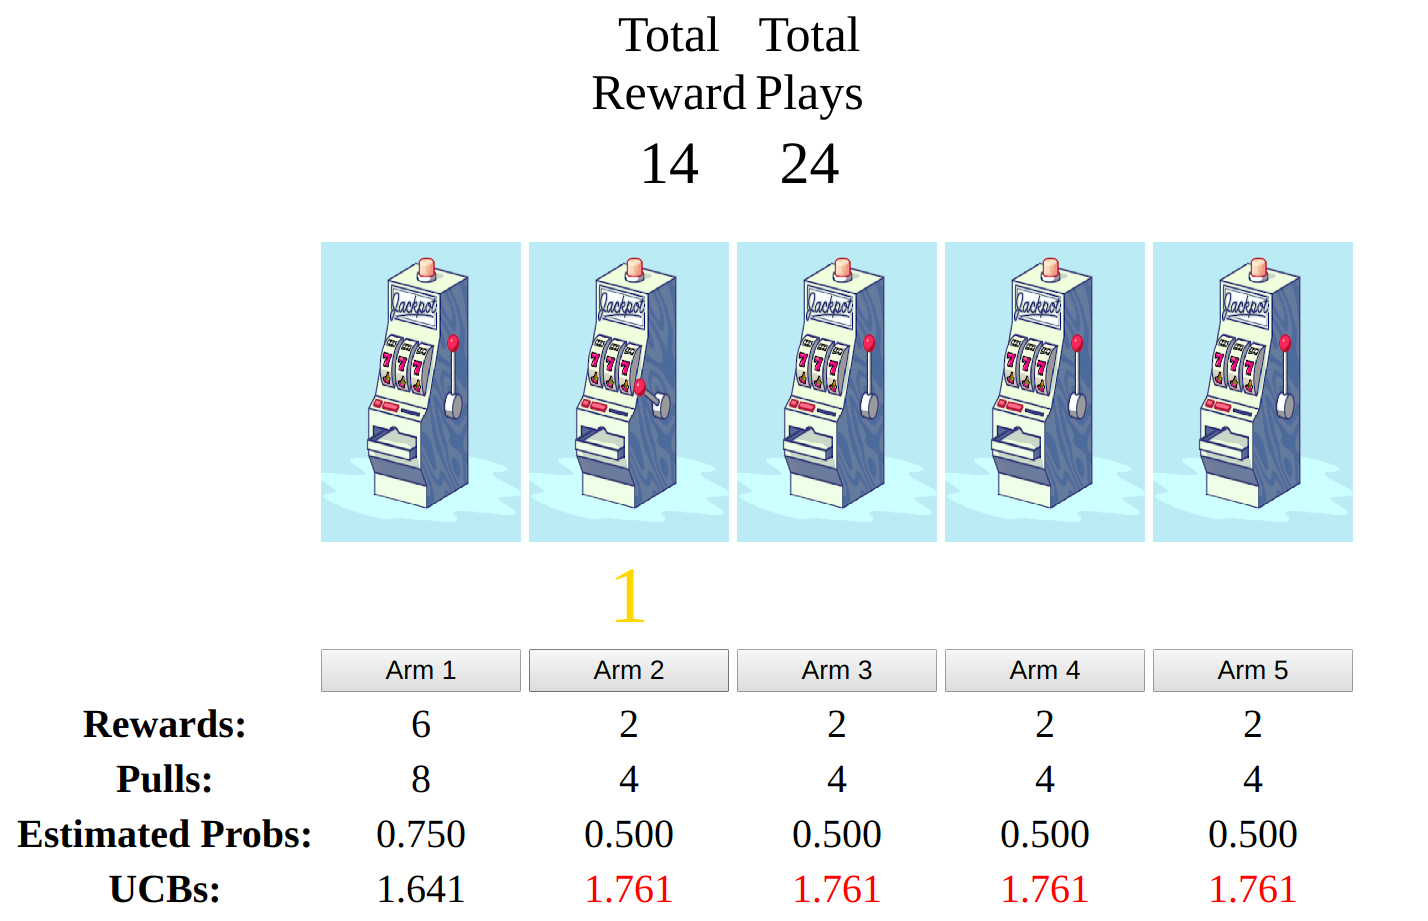
\includegraphics[height=0.55\textheight]{figures/example_of_a_5_arm_bandit_problem.png}
  \end{center}

  \begin{tiny}
  $\hookrightarrow$ Démo interactive
    \href{https://perso.crans.org/besson/phd/MAB_interactive_demo/}{\textcolor{blue}{\texttt{perso.crans.org/besson/phd/MAB\_interactive\_demo/}}}\\
    Réf : [Bandits Algorithms, Lattimore \& Szepesv{\'a}ri, 2019],
    sur \href{https://tor-lattimore.com/downloads/book/book.pdf}{\textcolor{blue}{\texttt{tor-lattimore.com/downloads/book/book.pdf}}}
  \end{tiny}

\end{frame}


\subsection{\hfill{}Modèle mathématique\hfill{}}

\begin{frame}{Modèle mathématique}

\begin{itemize}
  \item
  Étapes de temps discret $t = 1, \dots, T$\\
  L'\emph{horizon} $T$ est fixé et généralement inconnu

  \item
  Au temps $t$, une \emph{joueuse choisit le bras} $A(t)\in\{1,\dots,K\}$,\\
  et elle observe \emph{une récompense aléatoire iid} $r(t) \sim \nu_k$, $r(t)\in\mathbb{R}$

  \pause
  \item
  On se restreint souvent à des bras de Bernoulli $\nu_k = \mathrm{Bernoulli}(\mu_k)$, de moyenne $\mu_k\in[0,1]$,
  qui donnent des récompenses binaires $r(t) \in\{0,1\}$.

  \pause
  \item
  \textbf{But} : maximiser la somme des récompenses $\sum\limits_{t=1}^T r(t)$

  \item
  ou \alert{maximiser la somme des récompenses \emph{moyennes} $\mathbb{E}\left[ \sum\limits_{t=1}^T r(t) \right]$}

  \pause
  \item
  Une stratégie efficace doit résoudre le \alert{compromis entre exploration et exploitation} :
  explorer tous les bras pour découvrir le meilleur,
  tout en exploitant le meilleur bras courant.
\end{itemize}

\end{frame}


% \subsection{\hfill{}Naive solutions\hfill{}}

% \begin{frame}{Two examples of bad solutions}

%   \begin{exampleblock}{$i)$ Pure exploration \dXey{}}
%     \begin{itemize}
%       \item
%       Play arm $A(t) \sim \mathcal{U}(\{1,\dots,K\})$ uniformly at random
%       \item
%       $\implies$ Mean expected rewards
%       $ \frac{1}{T} \mathbb{E}\left[ \sum\limits_{t=1}^T r(t) \right] = \frac{1}{K} \sum\limits_{k=1}^K \mu_k \ll \max_k \mu_k$
%     \end{itemize}
%   \end{exampleblock}

%   \pause

%   \begin{exampleblock}{$ii)$ Pure exploitation \dXey{}}
%     \begin{itemize}
%       \item
%         Count the number of samples and the sum of rewards of each arm $N_k(t) = \sum\limits_{s < t} \mathbbm{1}(A(s)=k)$ and $X_k(t) = \sum\limits_{s < t} r(s) \mathbbm{1}(A(s)=k)$
%       \item
%         Estimate the \alert{unknown} mean $\mu_k$ with $\widehat{\mu_k}(t) = X_k(t) / N_k(t)$
%       \item
%         Play the arm of maximum empirical mean : $A(t) = \arg\max_k \widehat{\mu_k}(t)$
%       \item
%         Performance depends on the first draws, and can be very poor!
%     \end{itemize}
%   \end{exampleblock}
%   \vspace*{-10pt}
%   \begin{tiny}
%     $\hookrightarrow$
%     Interactive demo
%     \href{https://perso.crans.org/besson/phd/MAB_interactive_demo/}{\textcolor{blue}{\texttt{perso.crans.org/besson/phd/MAB\_interactive\_demo/}}}
%   \end{tiny}

% \end{frame}


% \subsection{\hfill{}The \emph{``Upper Confidence Bound''} algorithm\hfill{}}

% \begin{frame}{A first solution: \emph{``Upper Confidence Bound''} algorithm}

%   \begin{itemize}
%     \item
%       Compute $\mathrm{UCB}_k(t) = X_k(t) / N_k(t) + \sqrt{\alpha \log(t) / N_k(t)}$\\
%       $=$ an \alert{upper confidence bound} on the \alert{unknown} mean $\mu_k$
%     \item
%       Play the arm of maximal UCB : $A(t) = \arg\max_k \mathrm{UCB}_k(t)$
%       \\
%       $\hookrightarrow$ Principle of ``optimism under uncertainty''
%     \item
%       $\alpha$ balances between \emph{exploitation} ($\alpha\to0$) and \emph{exploration}  ($\alpha\to\infty$)

%     \pause

%     \item
%       \alert{UCB is efficient}:
%       the best arm is identified correctly (with high probability)
%       if there are enough samples (for $T$ large enough)
%     \item
%       $\implies$
%       Expected rewards attains the maximum \dLaughey{}
%       \[ \text{For~} T\to\infty, \;\;\; \frac{1}{T} \mathbb{E}\left[ \sum\limits_{t=1}^T r(t) \right] \to \max_k \mu_k \]
%   \end{itemize}
% \end{frame}

% \begin{frame}{UCB algorithm converges to the best arm}

%   We can prove that suboptimal arms $k$ are sampled about $o(T)$ times\\
%   $\implies \mathbb{E}\left[ \sum\limits_{t=1}^T r(t) \right] \underset{T\to\infty}{\to} \textcolor{deeppurple}{\mu^*} \times \mathcal{O}(T) + \sum\limits_{k: \Delta_k>0} \mu_k \times o(T)$
%   \dLaughey{}

%   \alert{But\ldots{} at which speed do we have this convergence?}

%   \begin{block}{Elements of proof of convergence (for $K$ Bernoulli arms)}
%     \begin{small}
%       \begin{itemize}
%         \item
%           Suppose the first arm is the best:
%           $\textcolor{deeppurple}{\mu^*} = \textcolor{deeppurple}{\mu_1} > \mu_2 \geq \ldots \geq \mu_K$
%         \item
%           $\mathrm{UCB}_k(t) = X_k(t) / N_k(t) + \sqrt{\alpha \log(t) / N_k(t)}$
%         \item
%           Hoeffding's inequality gives
%           $\mathbb{P}(\mathrm{UCB}_k(t) < \mu_k(t)) \leq \mathcal{O}(\frac{1}{t^{2 \alpha}})$\\
%           $\implies$ the different $\mathrm{UCB}_k(t)$ are true ``Upper Confidence Bounds'' on the (unknown) $\mu_k$ (most of the times)
%         \item
%           And if a suboptimal arm $k>\textcolor{deeppurple}{1}$ is sampled, it implies
%           $\mathrm{UCB}_k(t) > \mathrm{UCB}_{\textcolor{deeppurple}{1}}(t)$, but $\mu_k < \textcolor{deeppurple}{\mu_1}$:
%           Hoeffding's inequality also proves that any ``wrong ordering'' of the $\mathrm{UCB}_k(t)$ is unlikely
%         \end{itemize}
%       \end{small}
%     \end{block}

% \end{frame}


\subsection{\hfill{}Regret d'un algorithme de bandit\hfill{}}

\begin{frame}{Mesurer la performance d'un algorithme $\mathcal{A}$ par son regret moyen $R_{\mathcal{A}}(T)$}

\begin{itemize}
  \item
  Différence entre les récompenses accumulées par un ``oracle'' et $\mathcal{A}$

  \item
  L'algorithme ``oracle'' joue toujours \textcolor{deeppurple}{le meilleur bras (inconnu) $k^* = \arg\max_k \mu_k$} (la meilleure moyenne est notée \textcolor{deeppurple}{$\mu_{k^*} = \mu^*$})

  \item
  But équivalent : maximiser la somme des récompenses moyennes
  $\Longleftrightarrow$ \alert{minimiser le regret moyen}
  %
  \[ \alert{ R_{\mathcal{A}}(T) } = \mathbb{E}\left[ \sum\limits_{t=1}^T \textcolor{deeppurple}{r_{k^*}}(t) \right] - \sum\limits_{t=1}^T \mathbb{E}\left[ r(t) \right] = T \textcolor{deeppurple}{\mu^*} - \sum\limits_{t=1}^T \mathbb{E}\left[ r(t) \right]. \]

\end{itemize}

\pause
\vspace*{10pt}

\begin{exampleblock}{Régime typique pour des bandits stationnaires (bornes inf \& sup)}
  \begin{itemize}
  \item
  Aucun algorithme $\mathcal{A}$ ne peut atteindre un regret meilleur que
  \hfill{}
  $R_{\mathcal{A}}(T) \geq \Omega(\log(T))$

  \item
  Et un algorithme efficace $\mathcal{A}$ obtient
  \hfill{}
  $R_{\mathcal{A}}(T) \leq \mathcal{O}(\log(T))$
  \end{itemize}
\end{exampleblock}

\end{frame}

\subsection{\hfill{}Regret de deux algorithmes de type UCB\hfill{}}

\begin{frame}{Regret des algorithmes UCB et kl-UCB}

  Pour n'importe quel problème avec $K$ bras de Bernoulli, de moyennes $\mu_1,\dots,\mu_K \in[0,1]$, et de \textcolor{deeppurple}{bras optimal $\mu^*$} :

  \begin{exampleblock}{Pour l'algorithme UCB}
    \begin{small}
      \[ R_T^{\mathrm{UCB}} \leq \sum_{\substack{k=1,\dots,K \\ \mu_k < \textcolor{deeppurple}{\mu^*}}} \frac{8}{(\mu_k - \textcolor{deeppurple}{\mu^*})} \log(T) + o(\log(T)). \]
    \end{small}%
  \end{exampleblock}

  \begin{exampleblock}<2->{Pour l'algorithme kl-UCB : une meilleure borne}
    \begin{small}
      \[ R_T^{\mathrm{kl}\text{-}\mathrm{UCB}} \leq \sum_{\substack{k=1,\dots,K \\ \mu_k < \textcolor{deeppurple}{\mu^*}}} \frac{(\mu_k - \textcolor{deeppurple}{\mu^*})}{\mathrm{kl}(\textcolor{deeppurple}{\mu^*}, \mu_k)} \log(T) + o(\log(T)) = \mathcal{O}( \alert{\underbrace{C(\mu_1,\dots,\mu_K)}_{\text{Difficulté du problème}}} \log(T) ). \]
    \end{small}%
    \begin{footnotesize}
      Avec $\mathrm{kl}(x, y) = x \log(x/y) + (1-x) \log((1-x)/(1-y))$ l'\emph{entropie binaire relative}\\
      (\emph{ie}, la divergence de Kullback-Leibler de deux lois de Bernoulli de moyennes $x$ et $y$)
    \end{footnotesize}%
  \end{exampleblock}

\end{frame}


\section{\hfill{}2. Problèmes de bandits multi-bras stationnaires par morceaux\hfill{}}

\begin{frame}{2. Bandits stationnaires par morceaux}

  \begin{enumerate}
    \item
    \textcolor{gray}{
      Problèmes de bandits multi-bras (stationnaires)
    }
    \vspace*{15pt}

    \item
    \alert{\textbf{%
      Problèmes de bandits multi-bras stationnaires par morceaux
    }}
    \vspace*{15pt}

    \item
    \textcolor{gray}{
      Le test BGLR et ses propriétés à horizon fini
    }
    \vspace*{15pt}

    \item
    \textcolor{gray}{
      L'algorithme B-GLRT + klUCB
    }
    \vspace*{15pt}

    \item
    \textcolor{gray}{
      Analyse du regret
    }
    \vspace*{15pt}

    \item
    \textcolor{gray}{
      Simulations numériques
    }
  \end{enumerate}

\end{frame}


\begin{frame}{Problèmes de bandits non stationnaires}

  \begin{block}{Problèmes de bandits stationnaires}
    Le bras $k$ tire une récompense selon \textcolor{blue}{la même distribution} pour chaque instant :
    $\forall t, r_k(t) \overset{\text{iid}}{\sim} \nu_k = \mathrm{Bernoulli}(\mu_k)$.
  \end{block}

  \pause
  \begin{alertblock}{Problèmes de bandits \emph{non} stationnaires}
    Le bras $k$ tire une récompense selon \alert{une distribution différente à chaque instant} :
    $\forall t, r_k(t) \overset{\text{iid}}{\sim} \nu_k\alert{(t)} = \mathrm{Bernoulli}(\mu_k\alert{(t)})$.
  \end{alertblock}

  $\implies$ \dXey{} problème plus difficile !
  Et très difficile si $\mu_k(t)$ peut changer n'importe quand !

  \pause
  \begin{block}{Problèmes de bandits \textbf{stationnaires par morceaux}}
    $\hookrightarrow$ on se concentre sur le cas où il y a au plus $o(\sqrt{T})$ intervalles sur lesquels les moyennes sont toutes stationnaires (= \textbf{séquences})
  \end{block}
\end{frame}

\subsection{\hfill{}Définitions\hfill{}}

\begin{frame}{Ruptures et séquences stationnaires}

  On définit

  \begin{itemize}
    \item
    Le nombre de rupture\\
    $\Upsilon_T = \sum\limits_{t=1}^{T-1} \mathbbm{1}(\exists k\in \{1,\dots,K\}$ $:$ $\mu_k(t) \neq \mu_k(t+1) )$

    \item
    Le $i$ème point d'arrêt\\
    $\tau^{i} = \inf\{t > \tau^{i-1} : \exists k : \mu_k(t) \neq \mu_k(t+1)\}$
    \hfill{} (avec $\tau^0=0$)
  \end{itemize}

  \begin{block}<2->{\textbf{Hypothèses} sur les problèmes stationnaires par morceaux (p.m.)}
    \begin{itemize}\tightlist
      \item Les récompenses $r_k(t)$ générées par chaque bras $k$ sont \alert{\emph{iid} sur chaque intervale} $[ \tau^{i} + 1, \tau^{i+1} ]$ (la $i$ème séquence)
      \item Il y a $\Upsilon_T = o(\sqrt{T})$ ruptures
      \item Et \alert{$\Upsilon_T$ peut être connu à l'avance}
      \item Les séquences sont toutes ``assez longues``
  \end{itemize}
\end{block}
\end{frame}


\begin{frame}[plain]{Exemple d'un problème de bandits stationnaire p.m.}
  On affiche les moyennes \textcolor{red}{$\mu_1(t)$}, \textcolor{green}{$\mu_2(t)$}, \textcolor{blue}{$\mu_3(t)$}
  des $K=3$ bras.
  Il y a $\Upsilon_T=4$ ruptures, et $5$ séquences entre $t=1$ et $T=5000$ :
  \begin{center}
    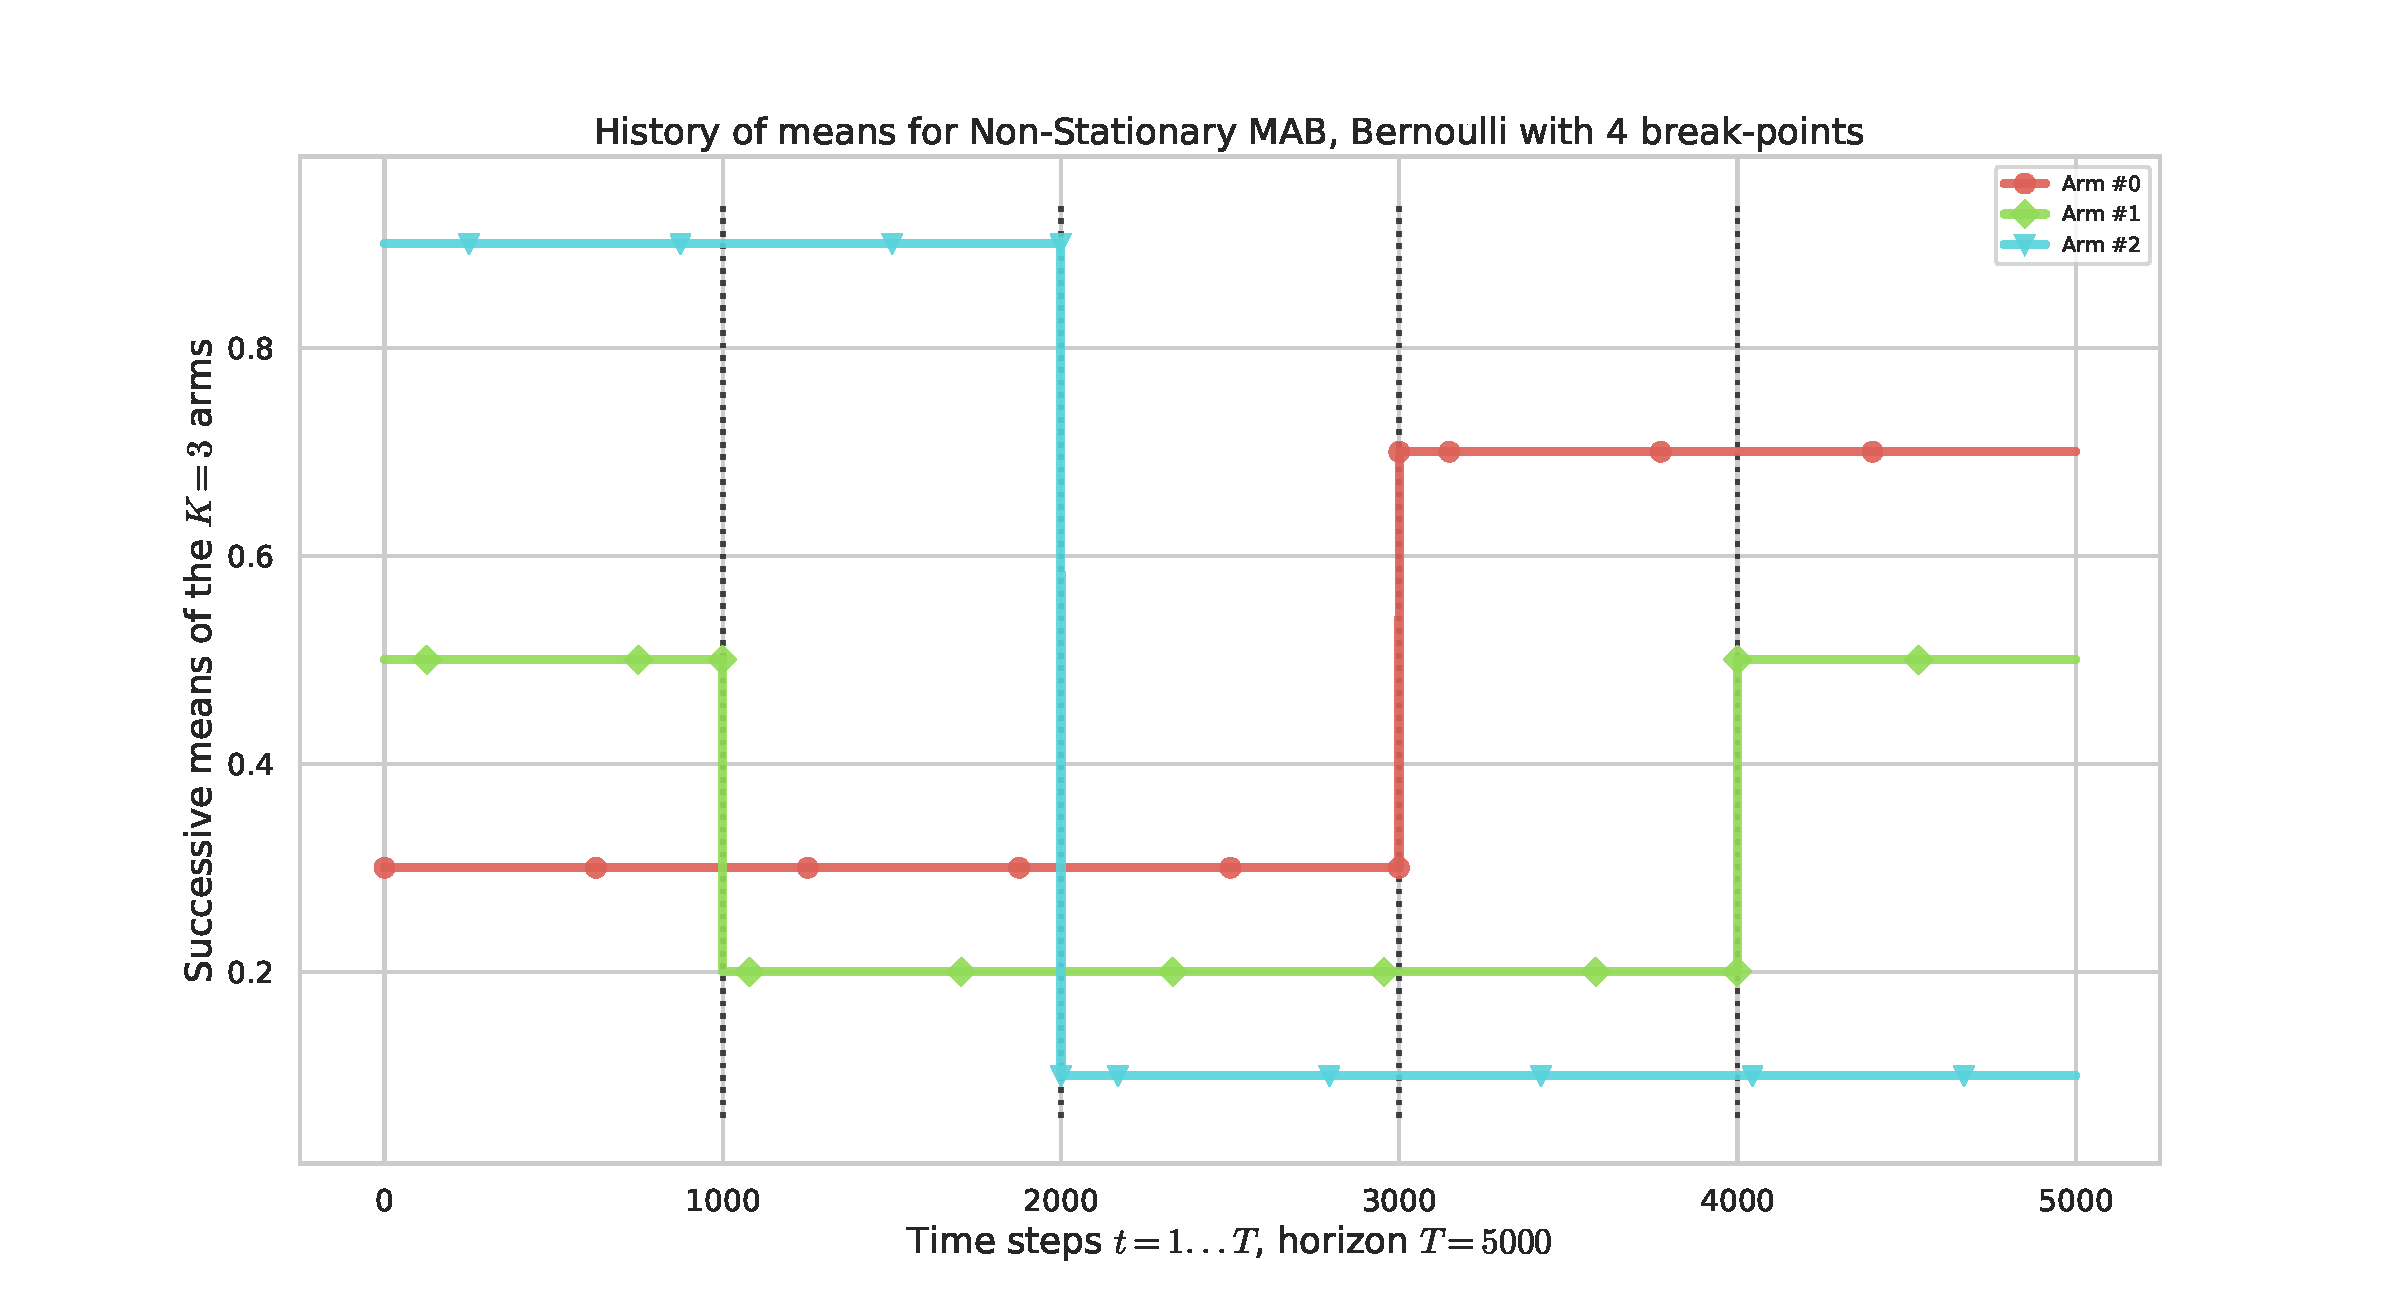
\includegraphics[width=1.00\textwidth]{figures/Problem_1.pdf}
  \end{center}
\end{frame}


\subsection{\hfill{}Étendre la définition du regret\hfill{}}

\begin{frame}{Regret pour les bandits stationnaires par morceaux ?}

  L'algorithme ``oracle'' joue le meilleur bras (inconnu) $k^*(t) = \arg\max \mu_k(t)$
  (qui change entre chaque séquence stationnaire)
  %
  \[ \alert{ R_{\mathcal{A}}(T) } = \mathbb{E}\left[ \sum\limits_{t=1}^T r_{\alert{k^*(t)}}(t) \right] - \sum\limits_{t=1}^T \mathbb{E}\left[ r(t) \right] = \left(\alert{\sum_{t=1}^T \max_k \mu_k(t)} \right) - \sum\limits_{t=1}^T \mathbb{E}\left[ r(t) \right]. \]

\pause
\vspace*{10pt}

\begin{exampleblock}{Régimes typiques pour les bandits stationnaires par morceaux}
  \begin{itemize}
  \item
  La borne inférieure est
  $R_{\mathcal{A}}(T) \geq \Omega(\sqrt{K T \Upsilon_T})$

  \item
  Actuellement, les meilleurs algorithmes $\mathcal{A}$  obtiennent
    \begin{itemize}\tightlist
      \item
      $R_{\mathcal{A}}(T) \leq \mathcal{O}(K \sqrt{T \Upsilon_T \log(T)})$
      si $T$ et $\Upsilon_T$ sont connus
      \item
      $R_{\mathcal{A}}(T) = \mathcal{O}(K \alert{\Upsilon_T} \sqrt{T \log(T)})$
      si $T$ et $\Upsilon_T$ sont inconnus
    \end{itemize}
  \end{itemize}
\end{exampleblock}

\end{frame}


\section{\hfill{}3. Le test BGLR et ses propriétés à horizon fini\hfill{}}

\begin{frame}{3. Le test BGLR et ses propriétés à horizon fini}

  \begin{enumerate}
    \item
    \textcolor{gray}{
      Problèmes de bandits multi-bras (stationnaires)
    }
    \vspace*{15pt}

    \item
    \textcolor{gray}{
      Problèmes de bandits multi-bras stationnaires par morceaux
    }
    \vspace*{15pt}

    \item
    \alert{\textbf{%
      Le test BGLR et ses propriétés à horizon fini
    }}
    \vspace*{15pt}

    \item
    \textcolor{gray}{
      L'algorithme B-GLRT + klUCB
    }
    \vspace*{15pt}

    \item
    \textcolor{gray}{
      Analyse du regret
    }
    \vspace*{15pt}

    \item
    \textcolor{gray}{
      Simulations numériques
    }
  \end{enumerate}

\end{frame}


\subsection{\hfill{}Détection de rupture\hfill{}}

\begin{frame}{Le problème de détection de rupture}

  Imaginez le problème suivants\ldots

  \begin{itemize}
    \item Vous observez des données $X_1,X_2,\cdots,X_t,\cdots \in[0,1]$\ldots
    \item Vous savez que $X_t$ est généré par une certaine distribution \alert{inconnue}\ldots

    \pause
    \item \alert{Votre but} est de distinguer entre deux hypothèses :
    \begin{itemize}
      \item[\textcolor{deeppurple}{$\mathcal{H}_0$}] \textcolor{deeppurple}{Les distributions \textbf{ont toutes la même moyenne} \hfill{} (``pas de rupture'')\\
      $\exists \mu_0, \mathbb{E}[X_1] = \mathbb{E}[X_2] = \cdots = \mathbb{E}[X_t] = \mu_0$}

      \item[\textcolor{gold}{$\mathcal{H}_1$}] \textcolor{gold}{Les distributions ont \textbf{changé de moyennes au temps $\tau$} \\
      $\exists \mu_0, \mu_1, \tau, \mathbb{E}[X_1] = \cdots = \mathbb{E}[X_{\tau}] = \mu_0, \; \mu_0 \neq \mu_1, \; \mathbb{E}[X_{\tau+1}] = \mathbb{E}[X_{\tau+2}] = \cdots = \mu_1$}
      % $\exists \mu_0, \mu_1, \exists \tau, \forall t \leq \tau, \mathbb{E}[X_t] = \mu_0 \text{ and } \forall t \geq \tau + 1, \mathbb{E}[X_t] = \mu_1$
    \end{itemize}
    \item Vous arrêtez au temps $\widehat{\tau}$, dès que vous détectez une rupture
  \end{itemize}

  \pause
  Un \alert{détecteur de rupture séquentiel} est un \alert{\textbf{temps d'arrêt $\widehat{\tau}$}},
  mesurable selon $\mathcal{F}_t = \sigma(X_1,\cdots,X_t)$,
  qui rejette l'hypothèse \textcolor{deeppurple}{$\mathcal{H}_0$}
  lorsque $\widehat{\tau} < \infty$.

\end{frame}


\subsection{\hfill{}Test de rapport de vraisemblance pour des données de Bernoulli\hfill{}}

\begin{frame}{Test de rapport de vraisemblance de Bernoulli}

  \textbf{Hypothèses} : toutes les distributions sont Bernoulli ($\nu_k = \mathcal{B}(\mu_k)$)

  Le problème se résume à distinguer
  \begin{itemize}
    \item[\textcolor{deeppurple}{$\mathcal{H}_0$}:]
    \textcolor{deeppurple}{$(\exists \mu_0 : \forall i\in\mathbb{N}^*, X_i \overset{\text{i.i.d.}}{\sim} \mathcal{B}(\mu_0))$},
    contre l'alternative
    \item[\textcolor{gold}{$\mathcal{H}_1$}:]
    \textcolor{gold}{$(\exists \mu_0 \neq \mu_1, \tau > 1 : X_1, \cdots, X_\tau \overset{\text{i.i.d.}}{\sim} \mathcal{B}(\mu_0) \text{~et~} X_{\tau+1}, \cdots \overset{\text{i.i.d.}}{\sim} \mathcal{B}(\mu_1))$}.
  \end{itemize}

  \pause

  Après avoir observé $X_1,\cdots,X_n$, la statistique du \alert{test de rapport de vraisemblances} pour cette hypothèse est
  \begin{small}
    \[ \mathcal{L}(n) = \frac{\sup\limits_{\textcolor{gold}{\mu_0,\mu_1,\tau < n}}\ell(X_1,\cdots,X_n ; \textcolor{gold}{\mu_0,\mu_1,\tau})}{\sup\limits_{\textcolor{deeppurple}{\mu_0}}\ell(X_1,\cdots,X_n ;\textcolor{deeppurple}{\mu_0})},\]
  \end{small}

  où $\ell(X_1,\cdots,X_n ; \textcolor{deeppurple}{\mu_0})$ (resp. $\ell(X_1,\cdots,X_n ; \textcolor{gold}{\mu_0,\mu_1,\tau})$) est la vraisemblance des observations selon le modèle \textcolor{deeppurple}{$\mathcal{H}_0$} (resp. \textcolor{gold}{$\mathcal{H}_1$}).

  \pause

  \alert{$\hookrightarrow$ De grandes valeurs de $\mathcal{L}(n)$ tendent à rejeter \textcolor{deeppurple}{$\mathcal{H}_0$} en faveur de \textcolor{gold}{$\mathcal{H}_1$}.}

\end{frame}

\begin{frame}{Expression du (log) rapport de vraisemblance de Bernoulli}

  On peut réécrire cette statistique
  $\mathcal{L}(n) = \frac{\sup\limits_{\textcolor{gold}{\mu_0,\mu_1,\tau < n}}\ell(X_1,\cdots,X_n ; \textcolor{gold}{\mu_0,\mu_1,\tau})}{\sup\limits_{\textcolor{deeppurple}{\mu_0}}\ell(X_1,\cdots,X_n ;\textcolor{deeppurple}{\mu_0})}$,
  en utilisant les vraisemblances de Bernoulli, et les moyennes glissantes $\widehat{\mu}_{k:k'} = \frac{1}{k'-k+1} \sum\limits_{s=k}^{k'} X_s$ :

  \begin{align*}
    \log \mathcal{L}(n) = \alert{\max_{s \in \{2,\cdots,n-1\}}} \bigl[
      & s \times \mathrm{kl} (\underbrace{\widehat{\mu}_{1:s}}_{\text{avant rupture}},\underbrace{\widehat{\mu}_{1:n}}_{\text{tout}} ) \\
      + & (n-s) \times \mathrm{kl} (\underbrace{\widehat{\mu}_{s+1:n}}_{\text{après rupture}},\underbrace{\widehat{\mu}_{1:n}}_{\text{tout}} ) \bigr].
  \end{align*}

  \begin{small}
    \textcolor{gray}{Où $\mathrm{kl}(x,y) =x \ln\bigl(\frac{x}{y}\bigr) + (1-x)\ln\bigl(\frac{1-x}{1-y}\bigr)$ est l'entropie relative binaire}
  \end{small}

\end{frame}


\subsection{\hfill{}Le B-GLRT\hfill{}}

\begin{frame}{Le test généralisé de rapport de vraisemblance de Bernoulli (B-GLRT)}

  \begin{itemize}
    \item
    On peut étendre ce test si les observations sont \alert{sous-Bernoulli}.
    ($=$ la fonction génératrice des moments est bornée par celle d'une loi de Bernoulli)
    \item
    Et toute distribution à support borné dans $[0,1]$ est sous-Bernoulli !
    \item
    $\implies$ le test B-GLR peut être appliqué à n'importe quelles observations bornées \dCooley{}
  \end{itemize}

  % \begin{block}{Sub-Bernoulli distributions}
  %   If $\nu$ is supported in $[0,1]$,
  %   $\nu$ is \emph{sub-Bernoulli} if it verifies
  %   $\mathbb{E}_{X\sim\nu}\left[e^{\lambda X}\right] \leq  1-\mu + \mu e^\lambda = \mathbb{E}_{X\sim \mathrm{Bernoulli}(\mu)} [e^{\lambda X}]$.
  %   % where $\mathcal{B}(\mu)$ est la loi de Bernoulli de moyenne $\mu$.
  % \end{block}

  \pause

  \begin{block}{Le test de détection séquentielle de rupture B-GRLT}
    Le \alert{B-GLRT} est le temps d'arrêt définit par
    \begin{small}
    \[ \widehat{\tau}_{\delta} = \inf \bigl\{ n \in \mathbb{N}^* : \max_{s \in \{2,\cdots,n-1\}} \bigl[s \, \mathrm{kl}\left(\widehat{\mu}_{1:s},\widehat{\mu}_{1:n}\right) + (n-s) \, \mathrm{kl}\left(\widehat{\mu}_{s+1:n},\widehat{\mu}_{1:n}\right)\bigr] \geq \beta(n,\delta) \bigr\} \]
    \vspace*{-10pt}
    \end{small}%
    \begin{itemize}\tightlist
      \item avec une \alert{function sueil} $\beta(n,\delta)$ spécifiée plus tard,
      \item $n$ est le nombre d'observations,
      \item $\delta$ est le niveau de confiance.
    \end{itemize}%
  \end{block}

\end{frame}


\subsection{\hfill{}Fausse alarme\hfill{}}

\begin{frame}{Probabilité de fausse alarme}

  Un bon test ne doit pas détecter de rupture s'il n'y a pas de rupture à détecter\ldots

  \pause
  \begin{block}{Définition : fausse alarme}
    Le temps d'arrêt est $\widehat{\tau}_\delta$,
    et une rupture est détectée si $\widehat{\tau}_\delta < \infty$.

    Soit $\mathbb{P}_{\textcolor{deeppurple}{\mu_0}}$ un modèle de probabilité selon lequel les observations sont $\forall t, X_t \in[0,1]$
    et \textcolor{deeppurple}{$\forall t, \mathbb{E}[X_t] = \mu_0$}.

    La \alert{probabilité de fausse alarme} est $\mathbb{P}_{\textcolor{deeppurple}{\mu_0}}(\widehat{\tau}_\delta < \infty)$.
  \end{block}

  \alert{$\implies$ But : contrôler l'événement de fausse alarme !} (en forte probabilité)

\end{frame}

\begin{frame}{First result for the BGLR test \dSmiley{}}

  \begin{block}{Controlling the false alarm probability}
    For any \alert{confidence level} $0<\delta<1$,
    the BGLR test satisfies
    \[ \mathbb{P}_{\textcolor{deeppurple}{\mu_0}}(\widehat{\tau}_\delta < \infty) \leq \delta \]
    with the threshold function
    \begin{small}
      \[ \beta(n,\delta) = \textcolor{gray}{2\,\mathcal{T}\left(\frac{\ln(3n\sqrt{n}/\delta)}{2}\right) + 6\ln(1+\ln(n))} \simeq \ln\left(\frac{3n \sqrt{n}}{\delta}\right) = \mathcal{O}\left(\log\left(\frac{n}{\delta}\right)\right).\]
    \end{small}
    \begin{footnotesize}
      \textcolor{gray}{Where $\mathcal{T}(x)$ verifies $\mathcal{T}(x)\simeq x + \ln(x)$ for $x$ large enough}
    \end{footnotesize}
  \end{block}


  \begin{exampleblock}<2>{Proof ?}
    Hard to explain in a short time\ldots\\
    %  we used time-uniform concentration inequalities
    $\hookrightarrow$ see the article, on
    \href{https://hal.inria.fr/hal-02006471}{\textcolor{blue}{HAL-02006471}}
    and
    \href{https://arxiv.org/abs/1902.01575}{\textcolor{blue}{arXiv:1902.01575}}
  \end{exampleblock}

\end{frame}

\subsection{\hfill{}Delay of detection\hfill{}}

\begin{frame}{Delay of detection}

  A good test should detect a break-point ``fast enough'' if there is a break-point to detect, with enough samples before the break-point\ldots

  \pause
  \begin{block}{Definition: Delay of detection}
    Let $\mathbb{P}_{\textcolor{gold}{\mu_0,\mu_1,\tau}}$ be a probability model under which $\forall t, X_t \in[0,1]$ and \textcolor{gold}{$\forall t \leq \tau, \mathbb{E}[X_t] = \mu_0$ and $\forall t \geq \tau + 1, \mathbb{E}[X_t] = \mu_1$,
    with $\mu_0 \neq \mu_1$}.

    The \alert{gap} of this break-point is $\Delta = |\mu_0 - \mu_1|$.

    The \alert{delay of detection} is $u = \widehat{\tau}_{\delta} - \tau \in\mathbb{N}$.
  \end{block}

  \alert{$\implies$ Goal: controlling the delay of detection!} (in high probability)

\end{frame}

\begin{frame}{Second result for the BGLR test \dSmiley{}}

  \begin{block}{Controlling the delay of detection}
      On a break-point of amplitude $\Delta = |\mu_1 - \mu_0|$,
      the BGLRT test satisfies
      \begin{small}
        \begin{align*}
            \mathbb{P}_{\textcolor{gold}{\mu_0,\mu_1,\tau}} (\widehat{\tau}_{\delta} \geq \textcolor{gold}{\tau} + u) &\leq \exp\left( -\frac{2\textcolor{gold}{\tau} u}{\textcolor{gold}{\tau} + u}\left(\max\left[ 0, \Delta - \sqrt{\frac{\textcolor{gold}{\tau} + u}{2\textcolor{gold}{\tau} u} \beta(\textcolor{gold}{\tau} + u,\delta)} \right]\right)^2 \right) \\
            &= \mathcal{O}(\text{decreasing exponential of~} u)
            = \mathcal{O}(\exp\searrow(u)).
        \end{align*}
      \end{small}
      with the same threshold function
      $\beta(n,\delta) \simeq \ln(3n \sqrt{n}/\delta)$.
  \end{block}

  \begin{exampleblock}{Consequence}
    In high probability, \alert{the delay $\widehat{\tau}_\delta$ of BGLR is bounded} by $\mathcal{O}(\Delta^{-2} \ln(1/\delta))$ \alert{if enough samples are observed before the break-point} at time $\tau$.
    % (at least $\mathcal{O}(\Delta^{-2} \ln(1/\delta))$ samples.
    % the detection delay of BGLR has the same magnitude.
  \end{exampleblock}

\end{frame}


\subsection{\hfill{}Summary of results for B-GLRT\hfill{}}

\begin{frame}{BGLR is an efficient break-point detection test \dCooley{} !}

  \begin{itemize}
    \item
    We just saw that by choosing
    \begin{itemize}\tightlist
      \item
      a confidence level $\delta$,
      \item
      and a good threshold function $\beta(n,\delta) \simeq \ln(3n \sqrt{n}/\delta) = \mathcal{O}(\log(n/\delta))$
    \end{itemize}
    \pause
    \item
    we can control the two properties of the BGLR test:
    \begin{itemize}\tightlist
      \item
        its \alert{false alarm probability}:
        $\mathbb{P}_{\textcolor{darkpurple}{\mu_0}}(\widehat{\tau}_\delta < \infty) \leq \delta$
      \item
        its \alert{detection delay}:
        $\mathbb{P}_{\textcolor{gold}{\mu_0,\mu_1,\tau}} (\widehat{\tau}_{\delta} \geq \tau + u)$ decreases exponentially fast wrt $u$
        (if there are enough samples before and after the break-point)
    \end{itemize}

    \item
    $\implies$ The BGLR is an efficient break-point detection test \dCooley{}
  \end{itemize}

  \pause
  \begin{block}{Finite time guarantees \dCooley{} \hfill{} \tiny{\textcolor{gray}{[Maillard, ALT, 2019]} \textcolor{gray}{[Lai \& Xing, Sequential Analysis, 2010]}}}
    Such \alert{finite time} (non asymptotic) guarantees are recent results!
  \end{block}

\end{frame}

\section{\hfill{}4. L'algorithme B-GLRT + klUCB\hfill{}}

\begin{frame}{4. L'algorithme B-GLRT + klUCB}

  \begin{enumerate}
    \item
    \textcolor{gray}{
      Problèmes de bandits multi-bras (stationnaires)
    }
    \vspace*{15pt}

    \item
    \textcolor{gray}{
      Problèmes de bandits multi-bras stationnaires par morceaux
    }
    \vspace*{15pt}

    \item
    \textcolor{gray}{
      Le test BGLR et ses propriétés à horizon fini
    }
    \vspace*{15pt}

    \item
    \alert{\textbf{%
      L'algorithme B-GLRT + klUCB
    }}
    \vspace*{15pt}

    \item
    \textcolor{gray}{
      Analyse du regret
    }
    \vspace*{15pt}

    \item
    \textcolor{gray}{
      Simulations numériques
    }
  \end{enumerate}

\end{frame}

\subsection{\hfill{}BGRL test + kl-UCB index\hfill{}}

\begin{frame}{Our algorithm combines BGRL test + kl-UCB index}

  \begin{block}{Main ideas}
    \begin{itemize}
      % \item Forced uniform random exploration with probability $\alpha$
      \item We compute a UCB index on each arm $k$
        % $\mbox{kl-UCB}_k(t)$
      \item Most of the times, we select
      $A(t) = \arg\max\limits_{k\in \{1,\dots,K\}} \mbox{kl-UCB}_k(t)$
      \item We use a BGLR test \alert{to detect changes on the played arm $A(t)$}
      \item If a break-point is detected, \alert{we reset the memories of \emph{all arms}}
    \end{itemize}
  \end{block}

  \pause

  \begin{exampleblock}{The kl-UCB indexes}
    \begin{itemize}
      \item $\tau_k(t)$ is the time of last reset of arm $k$ before time $t$,
      \item $n_k(t)$ counts the selections and $\widehat{\mu}_k(t)$ is the empirical means of observations of arm $k$ since $\tau_k(t)$,
      % = \sum\limits_{s=\tau_k(t)+1}^{t} \mathbbm{1}(A_s=k)$
      % la moyenne empirique des récompenses obtenues entre la dernière réinitialisation et l'instant $t$.
      %= (\sum_{s=\tau_i(t)+1}^{t}X_{i,s} \mathbbm{1}(A_s=i))/n_i(t)$ (si $n_i(t)\neq0$)
      \item Let {\small $\mbox{kl-UCB}_k(t) = \max \bigl\{ q\in[0,1] : n_k(t) \times \mathrm{kl}\left(\widehat{\mu}_k(t),q\right) \leq f(t - \tau_k(t)) \bigr\}$ }
      \item $f(t) = \ln(t) + 3 \ln(\ln(t))$ controls the width of the UCB.
    \end{itemize}
  \end{exampleblock}

\end{frame}

\begin{frame}{Two details of our algorithm}

  % % \GLRklUCB{} repose sur le calcul d'un \emph{indice} (de type \mathrm{kl}UCB{} \cite{KLUCBJournal}) pour chaque bras,  et choisit en général le bras d'indice le plus élevé.
  % Soit $\tau_i(t)$ l'instant de la dernière réinitialisation pour le bras $i$ avant le temps $t$, $n_i(t) = \sum_{s=\tau_i(t)+1}^{t} \mathbbm{1}(A_s=i)$ le nombre de sélections et $\widehat{\mu}_i(t)$
  % %= (\sum_{s=\tau_i(t)+1}^{t}X_{i,s} \mathbbm{1}(A_s=i))/n_i(t)$ (si $n_i(t)\neq0$)
  % la moyenne empirique des récompenses obtenues entre la dernière réinitialisation et l'instant $t$.

  % % L'indice du bras $i$ à l'instant $t$ est défini par
  % % $\UCB_i(t) = \max \bigl\{ q\in[0,1] : n_i(t) \times \mathrm{kl}\left(\widehat{\mu}_i(t),q\right) \leq f(t - \tau_i(t)) \bigr\}$ (l. $6$) avec la fonction d'exploration $f(t) = \ln(t) + 3 \ln(\ln(t))$.
  % % La détection d'une rupture sur le bras qui vient d'être joué
  % % produit une réinitialisation (l. $12$),

  \begin{exampleblock}{$i)$ How do we use the BGLR test? \hfill{} (parameter $\delta$)}
    From observations $Z_1,\cdots,Z_n$
    % $\mbox{BGLRT}_\delta(Z_1,\dots,Z_n) = \mathrm{True}$
    we use the BGLR test to detect a break-point
    with confidence level $\delta$
    when
    % \begin{footnotesize}
      \[
        \sup_{2 \leq s \leq n-1} \left[s \times \mathrm{kl} \left( \widehat{Z}_{1:s}, \widehat{Z}_{1:n}\right) + (n-s) \times \mathrm{kl} \left( \widehat{Z}_{s+1:n}, \widehat{Z}_{1:n} \right) \right] \geq \beta(n,\delta)
        \]
    % \end{footnotesize}%
    % We use $\beta(n,\delta) \simeq \ln(3n^{3/2}/\delta)$
  \end{exampleblock}

  \pause

  \begin{exampleblock}{$ii)$ Forced exploration \hfill{} (parameter $\alpha$)}
    \begin{itemize}
      \item We use a forced exploration uniformly on all arms\ldots\\
        \emph{ie}, in average, arm $k$ is forced to be sampled at least $T \times \alpha / K$ times
      \item $\implies$ so we can detect break-points on all the arms
      \item and not only on the arm played by the kl-UCB indexes
      % (lignes $5$-$6$), qui assure que chaque bras est suffisamment échantillonné, afin que les ruptures puissent aussi être détectées sur les bras actuellement sous-échantillonnés par l'algorithme de bandit.
    \end{itemize}
  \end{exampleblock}

\end{frame}

\begin{frame}{The \textcolor{gold}{BGLR} + \textcolor{deeppurple}{kl-UCB} algorithm}

\begin{columns}
\begin{column}{0.02\textwidth}
  %
\end{column}
\begin{column}{0.97\textwidth}
\begin{footnotesize}
  % Documentation at http://mirror.ctan.org/tex-archive/macros/latex/contrib/algorithm2e/doc/algorithm2e.pdf if needed
  % Or https://en.wikibooks.org/wiki/LaTeX/Algorithms#Typesetting_using_the_algorithm2e_package
  \removelatexerror% Nullify \@latex@error % Cf. http://tex.stackexchange.com/a/82272/
  \begin{algorithm}[H]
      % XXX Options
      % \LinesNumbered  % XXX Option to number the line
      % \RestyleAlgo{boxed}
      % XXX Input, data and output
      \KwData{\emph{Parameters of the problem} : $T\in\mathbb{N}^*$, $K\in\mathbb{N}^*$}
      \KwData{\emph{Parameters of the algorithm} : $\alpha \in (0, 1)$, $\delta>0$ \tcp*[f]{can use $T$ and $\Upsilon_T$}}
      % \KwData{\emph{Option} : redémarrages \textbf{Locaux} ou \textbf{Globaux}\;}
      % \KwData{Data}
      % \KwResult{Result}
      % XXX Algorithm
      \textbf{Initialisation : } $\forall k \in \{1,\dots,K\}$, $\tau_k = 0$ and $n_k = 0$ \\
      \For{$t=1,2,\ldots, T$}{
          \pause
          \uIf{
              $t \mod \left\lfloor \frac{K}{\alpha}\right\rfloor \in \{1,\dots,K\}$
          }{
              $A(t) = t \mod \left\lfloor \frac{K}{\alpha}\right\rfloor$
              \tcp*[f]{forced exploration} \\
          }
          \uElse{
            \textcolor{deeppurple}{$A(t) = \arg\max\limits_{k\in \{1,\dots,K\}} \mbox{kl-UCB}_k(t)$}
              \tcp*[f]{\textcolor{deeppurple}{highest UCB index}}
          }
          \pause
          \mbox{Play arm} $k=A(t)$, and update play count $n_{A(t)} = n_{A(t)} + 1$ \\
          \mbox{Observe a reward} $X_{A(t),t}$, and store it $Z_{A(t), n_{A(t)}} = X_{A(t),t}$ \\
          \pause
          \uIf{
            \textcolor{gold}{$\mathrm{BGLRT}_\delta(Z_{A(t),1}, \cdots, Z_{A(t), n_{A(t)}})$ = True}
          }
          {
              % \uSi{Redémarrages \textbf{globaux}}{
                \textcolor{gold}{$\forall k, \tau_k = t$ and $n_k = 0 $}
                \tcp*[f]{\textcolor{gold}{reset memories of all arms}}
                  % \tcp*[f]{redémarrages globaux}
                  % }
              % \Sinon{
                  % $\tau_{A(t)} = t$ and $n_{A(t)} = 0$
                  % \tcp*[f]{redémarrage local}
              % }
          }
      }
  \end{algorithm}
\end{footnotesize}

\end{column}
\end{columns}

\end{frame}


\section{\hfill{}5. Analyse du regret\hfill{}}

\begin{frame}{5. Analyse du regret}

  \begin{enumerate}
    \item
    \textcolor{gray}{
      Problèmes de bandits multi-bras (stationnaires)
    }
    \vspace*{15pt}

    \item
    \textcolor{gray}{
      Problèmes de bandits multi-bras stationnaires par morceaux
    }
    \vspace*{15pt}

    \item
    \textcolor{gray}{
      Le test BGLR et ses propriétés à horizon fini
    }
    \vspace*{15pt}

    \item
    \textcolor{gray}{
      L'algorithme B-GLRT + klUCB
    }
    \vspace*{15pt}

    \item
    \alert{\textbf{%
      Analyse du regret
    }}
    \vspace*{15pt}

    \item
    \textcolor{gray}{
      Simulations numériques
    }
  \end{enumerate}

\end{frame}

\subsection{\hfill{}Hypotheses\hfill{}}

\begin{frame}{Hypotheses of our theoretical analysis}

  \begin{itemize}
    \item
    Denote $\tau^{i}$ the position of break-point $i$ ($\tau^0 = 0$)
    \item
    and $\mu_k^{i}$ the mean of arm $k$ on the segment $[\tau^i, \tau^{i+1}]$
    \item
    and $b(i) \in \arg\max_k \mu_k^{i}$ (one of) the best arm(s) on the $i$-th segment
    \item
    and the largest gap at break-point $i$ is
    $\Delta^{i} = \max\limits_{k=1,\dots,K} |\mu_k^{i} - \mu_k^{i-1}| >0$
  \end{itemize}

  \pause
  \begin{block}{Assumption}
    Fix the parameters $\alpha$ and $\delta$,
    and let $d^{i} = d^{i}(\alpha,\delta) = \lceil \frac{4K}{\alpha(\Delta^{i})^2}\beta(T,\delta) + \frac{K}{\alpha} \rceil$.

    \alert{\textbf{We assume that all sequences are ``long enough'':}}
    \vspace*{-5pt}
    \[ \forall i \in \{1,\dots,\Upsilon_T\}, \;\;\;\; \alert{\tau^{i} - \tau^{i-1}} \geq 2\max( d^{i}, d^{i-1} ). \]
  \end{block}

  \pause
  $\hookrightarrow$
  The \alert{minimum length of sequence $i$} depends on the amplitude of the changes at \textcolor{darkred}{the beginning} and \textcolor{darkblue}{the end} of the sequence (\textcolor{darkred}{$\Delta^{i-1}$} and \textcolor{darkblue}{$\Delta^{i}$}).

\end{frame}


\subsection{\hfill{}Regret upper-bound\hfill{}}

\begin{frame}{Theoretical result}

  Under this hypothesis, we obtained a \emph{finite time}
  upper-bound on the regret $R_T$,
  with explicit dependency from the problem difficulty.

  The exact bound uses:
  \begin{itemize}
    \item
    the divergences $\mathrm{kl}(\mu_{k}^{i},\mu_{b(i)}^{i})$
    account for the difficulty of the stationary problem on sequence $i$,
    \item
    the gaps $\Delta^{i}$
    account for the difficulty of detecting break-point $i$,
  \end{itemize}
  as well as the two parameters
  \begin{itemize}
    \item
    $\alpha$ the probability of forced exploration,
    \item
    and $\delta$ the confidence level of the break-point detection test.
  \end{itemize}

\end{frame}


\begin{frame}{Simplified form of the result for \textcolor{gold}{BGLR} + \textcolor{deeppurple}{kl-UCB}}

  \begin{block}{Regret upper bound for BGLR + kl-UCB \dCooley{}}
    \begin{itemize}
      \item
      On a problem satisfying our assumption\ldots
      \item
      let $\alpha = \sqrt{\Upsilon_T \ln(T) / T}$ and $\delta = 1 / \sqrt{T \Upsilon_T}$ (if $T$ and $\Upsilon_T$ are known),
      \pause
      \item
      then if BGLR + kl-UCB uses parameters $\alpha$ and $\delta$, its regret satisfies
      %
      \[ R_T =\mathcal{O}\left( \frac{K}{\left(\textcolor{gold}{\Delta^{\text{change}}}\right)^2}\sqrt{T \Upsilon_T \ln(T)} + \frac{(K-1)}{\textcolor{deeppurple}{\Delta^{\text{opt}}}} \Upsilon_T\ln(T) \right),\]
      \begin{itemize}\tightlist
        \item
        with $\textcolor{gold}{\Delta^{\text{change}}} =$
        %  $\min_{i} \Delta^{i} =$
        \textcolor{gold}{the smallest detection gap between two stationary segments}
        $=$ \textcolor{gold}{Difficulty of the break-point detection problems!}
        \item
        and $\textcolor{deeppurple}{\Delta^{\text{opt}}} =$
        \textcolor{deeppurple}{the smallest value of sub-optimality gap on a stationary segment}
        $=$ \textcolor{deeppurple}{Difficulty of the stationary bandit problems!}
      \end{itemize}
      % ($\min_{k: \mu_k(t) < \mu_{k^*(t)}(t)} \mu_{k^*(t)}(t) - \mu_k(t)$)
    \end{itemize}
  \end{block}

\pause
$\implies$ $R_T = \mathcal{O}(K \sqrt{T \Upsilon_T \log(T)})$ if we hide the dependency on the gaps.

\end{frame}


\subsection{\hfill{}Comparison with other algorithms\hfill{}}

\begin{frame}{Comparison with other state-of-the-art approaches}

  \begin{exampleblock}{Our algorithm (BGLR + kl-UCB)}
    \begin{itemize}
      \item Hypotheses: bounded rewards, known $T$, known $\Upsilon_T = o(\sqrt{T})$, and ``long enough'' stationary sequences
      \item We obtain $R_T = \mathcal{O}(K \sqrt{T \Upsilon_T \log(T)})$
    \end{itemize}
  \end{exampleblock}

  \pause
  Two recent competitors
  use a similar assumption
  \alert{but they both require prior knowledge of a lower-bound on the gaps}

  % \begin{block}{Exp3.S \hfill{} \textcolor{gray}{[Auer et al, 2002]}}
  %   \begin{itemize}
  %     \item Hypotheses: just bounded rewards
  %     \item $R_T = \mathcal{O}(K \sqrt{T \Upsilon_T})$
  %     \item But usually poor in practice
  %   \end{itemize}
  % \end{block}

  \begin{block}{CUSUM-UCB \hfill{} \textcolor{gray}{[Liu \& Lee \& Shroff, AAAI 2018]}}
    \begin{itemize}
      \item They obtain $R_T = \mathcal{O}(K \sqrt{T \Upsilon_T \log(T / \Upsilon_T)})$
    \end{itemize}
  \end{block}

  \begin{block}{M-UCB \hfill{} \textcolor{gray}{[Cao \& Zhen \& Kveton \& Xie, AISTATS 2019]}}
    \begin{itemize}
      \item They obtain $R_T = \mathcal{O}(K \sqrt{T \Upsilon_T \log(T)})$
    \end{itemize}
  \end{block}

\end{frame}


\section{\hfill{}6. Simulations numériques\hfill{}}

\begin{frame}{6. Simulations numériques}

  \begin{enumerate}
    \item
    \textcolor{gray}{
      Problèmes de bandits multi-bras (stationnaires)
    }
    \vspace*{15pt}

    \item
    \textcolor{gray}{
      Problèmes de bandits multi-bras stationnaires par morceaux
    }
    \vspace*{15pt}

    \item
    \textcolor{gray}{
      Le test BGLR et ses propriétés à horizon fini
    }
    \vspace*{15pt}

    \item
    \textcolor{gray}{
      L'algorithme B-GLRT + klUCB
    }
    \vspace*{15pt}

    \item
    \textcolor{gray}{
      Analyse du regret
    }
    \vspace*{15pt}

    \item
    \alert{\textbf{%
      Simulations numériques
    }}
  \end{enumerate}

\end{frame}


\subsection{\hfill{}Setup of the experiments\hfill{}}

\begin{frame}{Simulations numériques}

  \begin{block}{We consider three problems with}
    \begin{itemize}
      \item
      $K=3$ arms, Bernoulli distributed
      \item
      $T=5000$ time steps (fixed horizon)
      \item
      $\Upsilon_T=4$ break-points ($=5$ stationary sequences)\\
      Algorithms can use this prior knowledge of $T$ and $\Upsilon_T$
      \item
      $1000$ independent runs, we plot the average regret
    \end{itemize}
  \end{block}

  \pause

  \begin{exampleblock}{Reference}
    \begin{itemize}
      \item
      We used my open-source Python library for simulations of multi-armed bandits problems, \textbf{SMPyBandits}
      \\
      $\hookrightarrow$ Published online at \href{https://SMPyBandits.GitHub.io}{\textcolor{blue}{\texttt{SMPyBandits.GitHub.io}}}
      \item
      More experiments are included in the long version of the paper!\\
      $\hookrightarrow$ pre-print on
      \href{https://hal.inria.fr/hal-02006471}{\textcolor{blue}{HAL-02006471}}
      and
      \href{https://arxiv.org/abs/1902.01575}{\textcolor{blue}{arXiv:1902.01575}}
    \end{itemize}
  \end{exampleblock}

\end{frame}


\begin{frame}[plain]{Problem 1: only local changes}
  \centering
  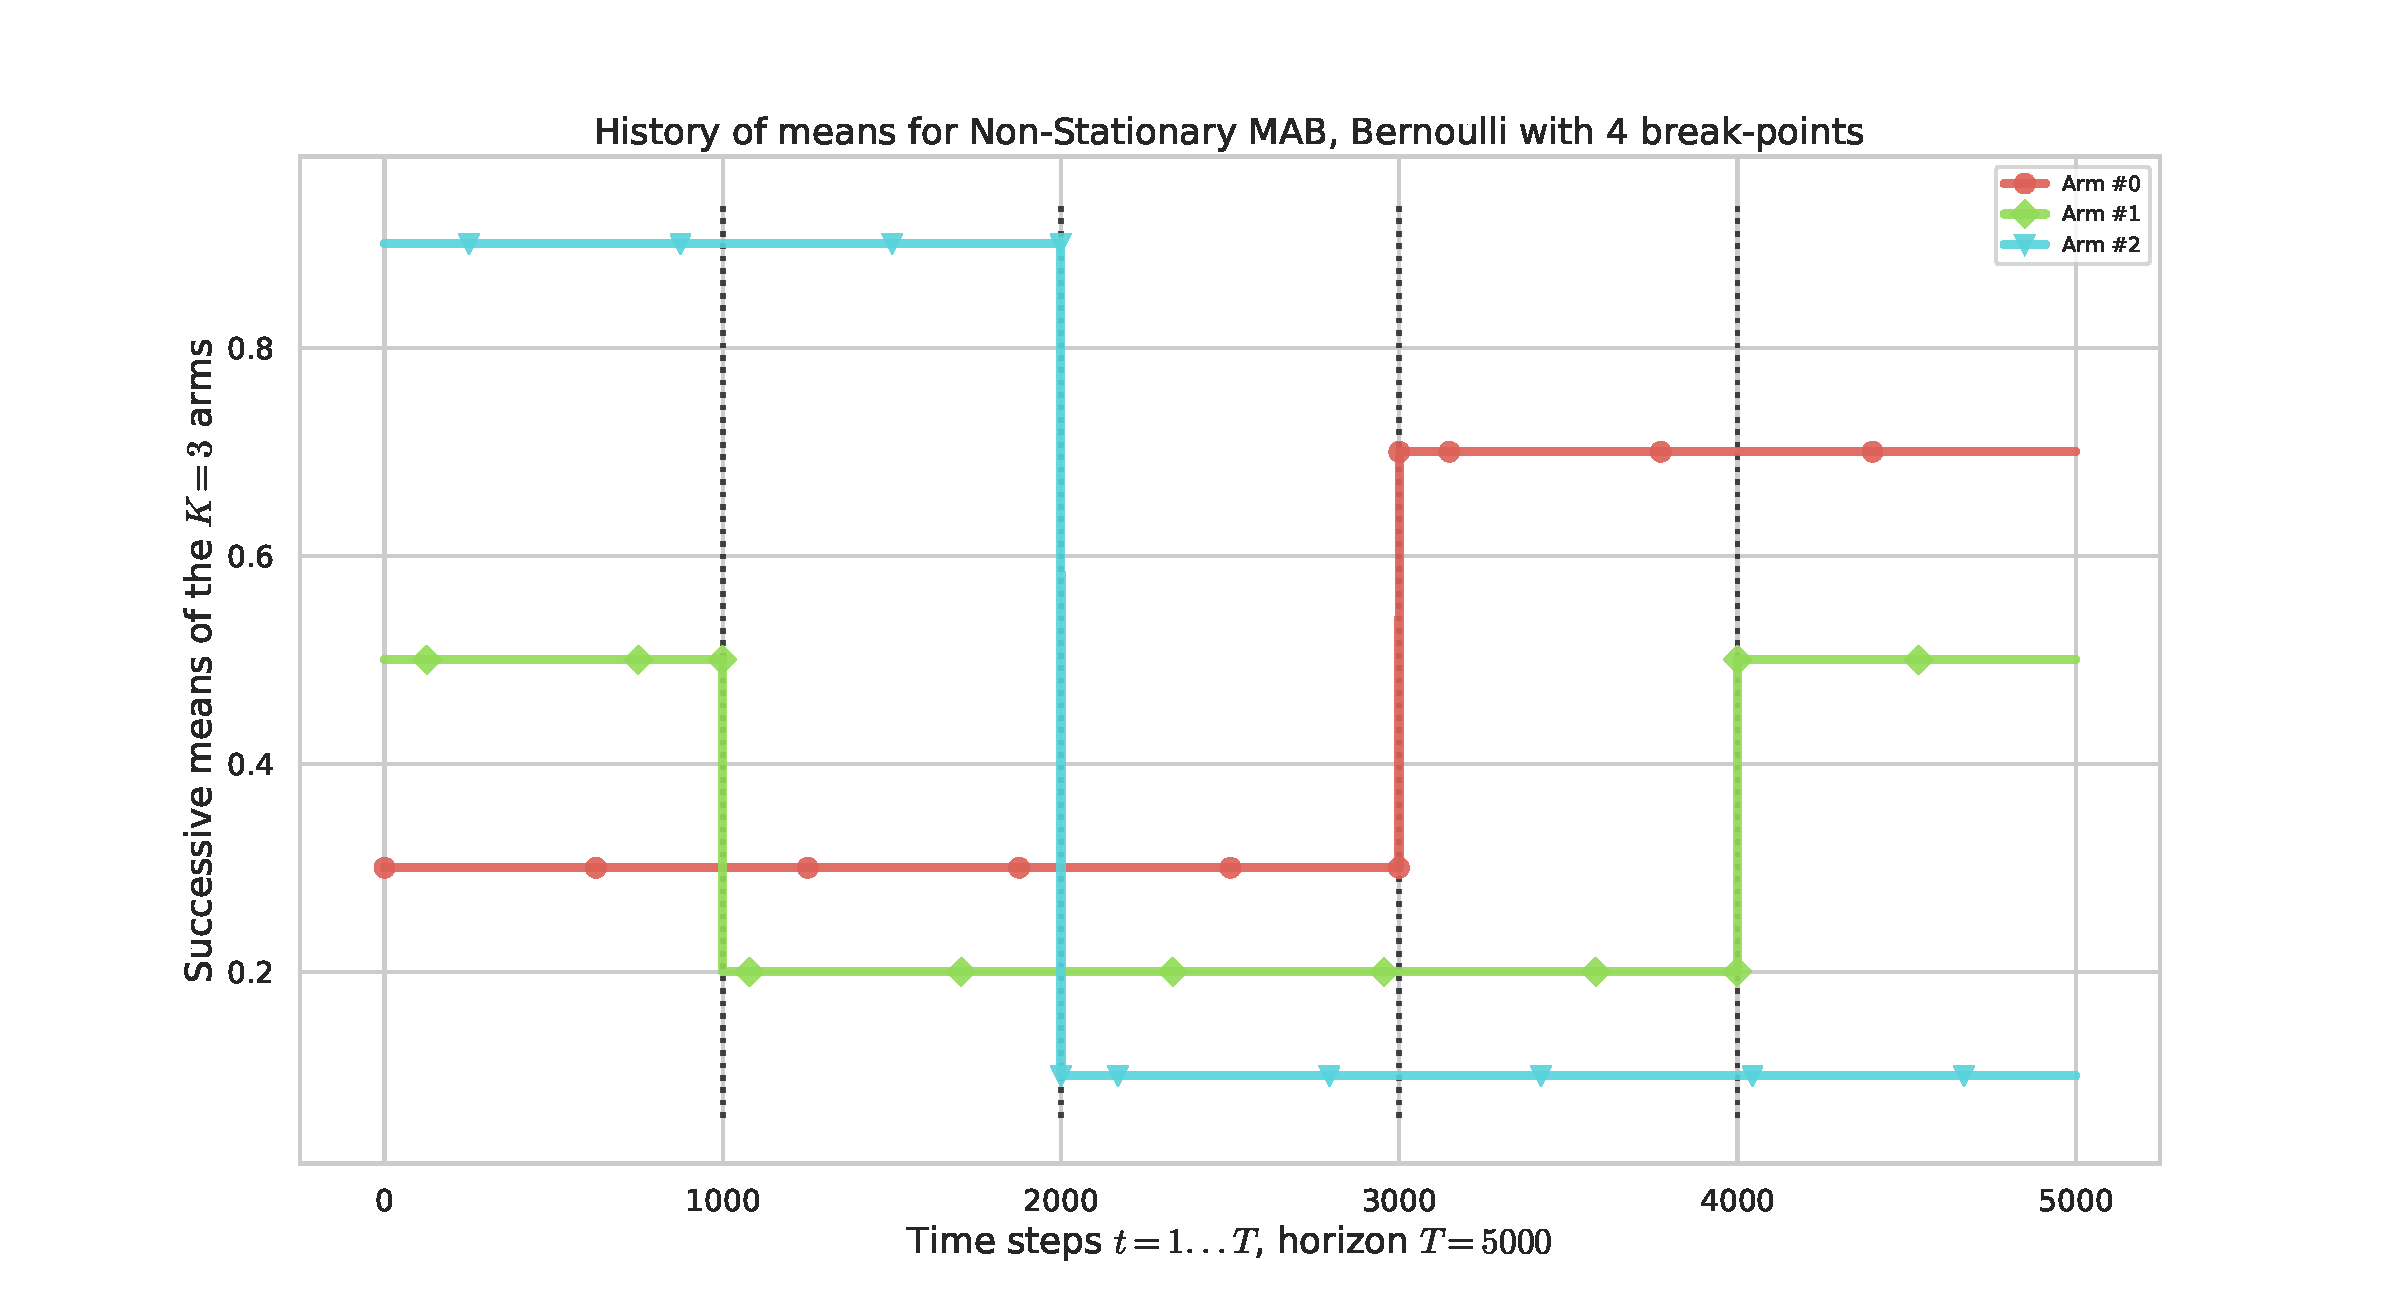
\includegraphics[width=1.00\textwidth]{figures/Problem_1.pdf}

  We plots the means:
  \textcolor{red}{$\mu_1(t)$},
  \textcolor{green}{$\mu_2(t)$},
  \textcolor{blue}{$\mu_3(t)$}.
\end{frame}

\begin{frame}[plain]{Results on problem 1}
  \centering
  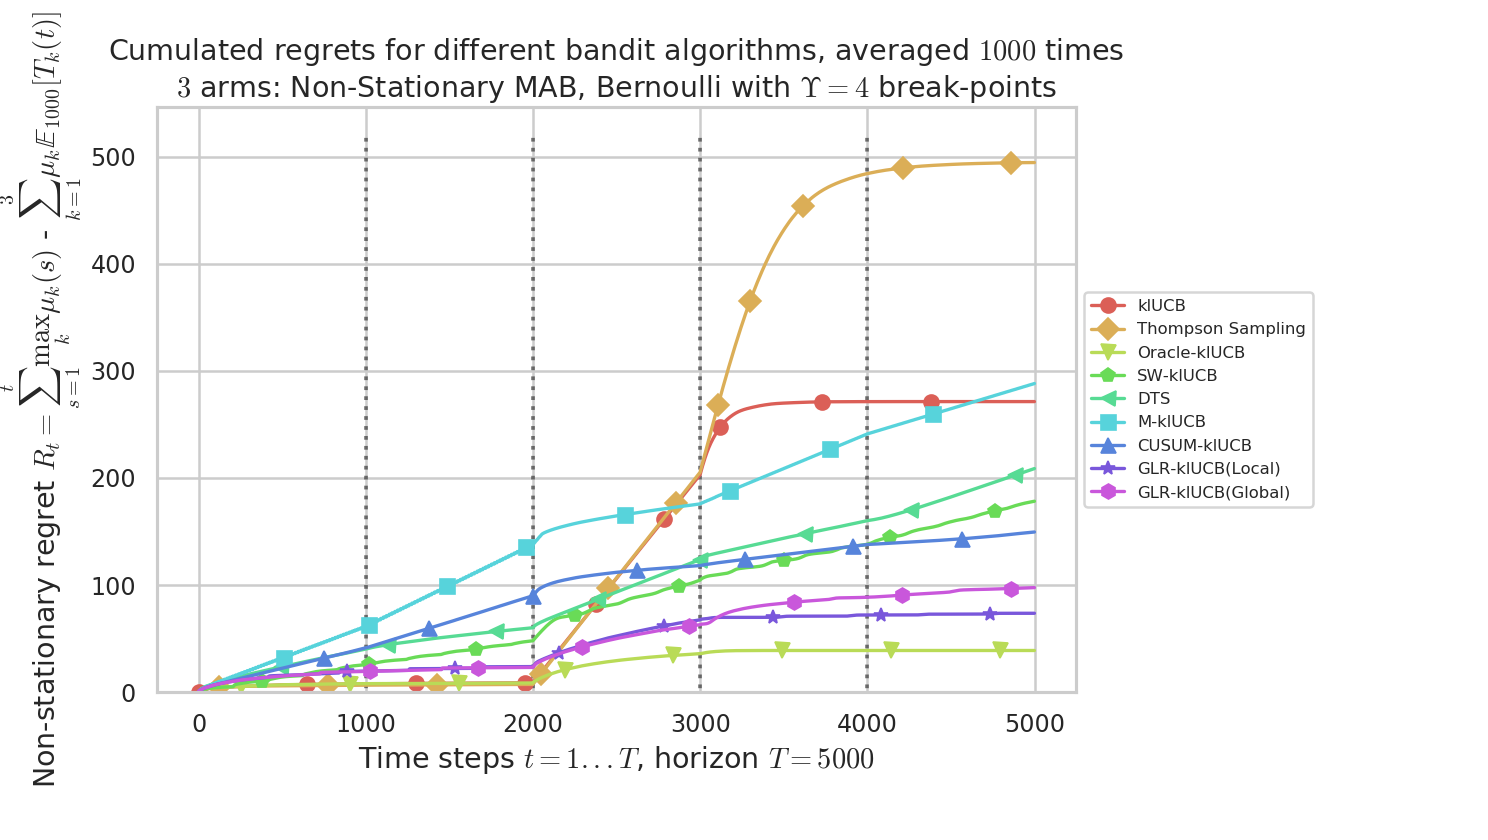
\includegraphics[width=1.05\textwidth]{figures/regret_problem1.png}

  $\implies$ BGLR achieves the best performance among non-oracle algorithms \dCooley{} !
\end{frame}


\begin{frame}[plain]{Problem 2: only global changes}
  \centering
  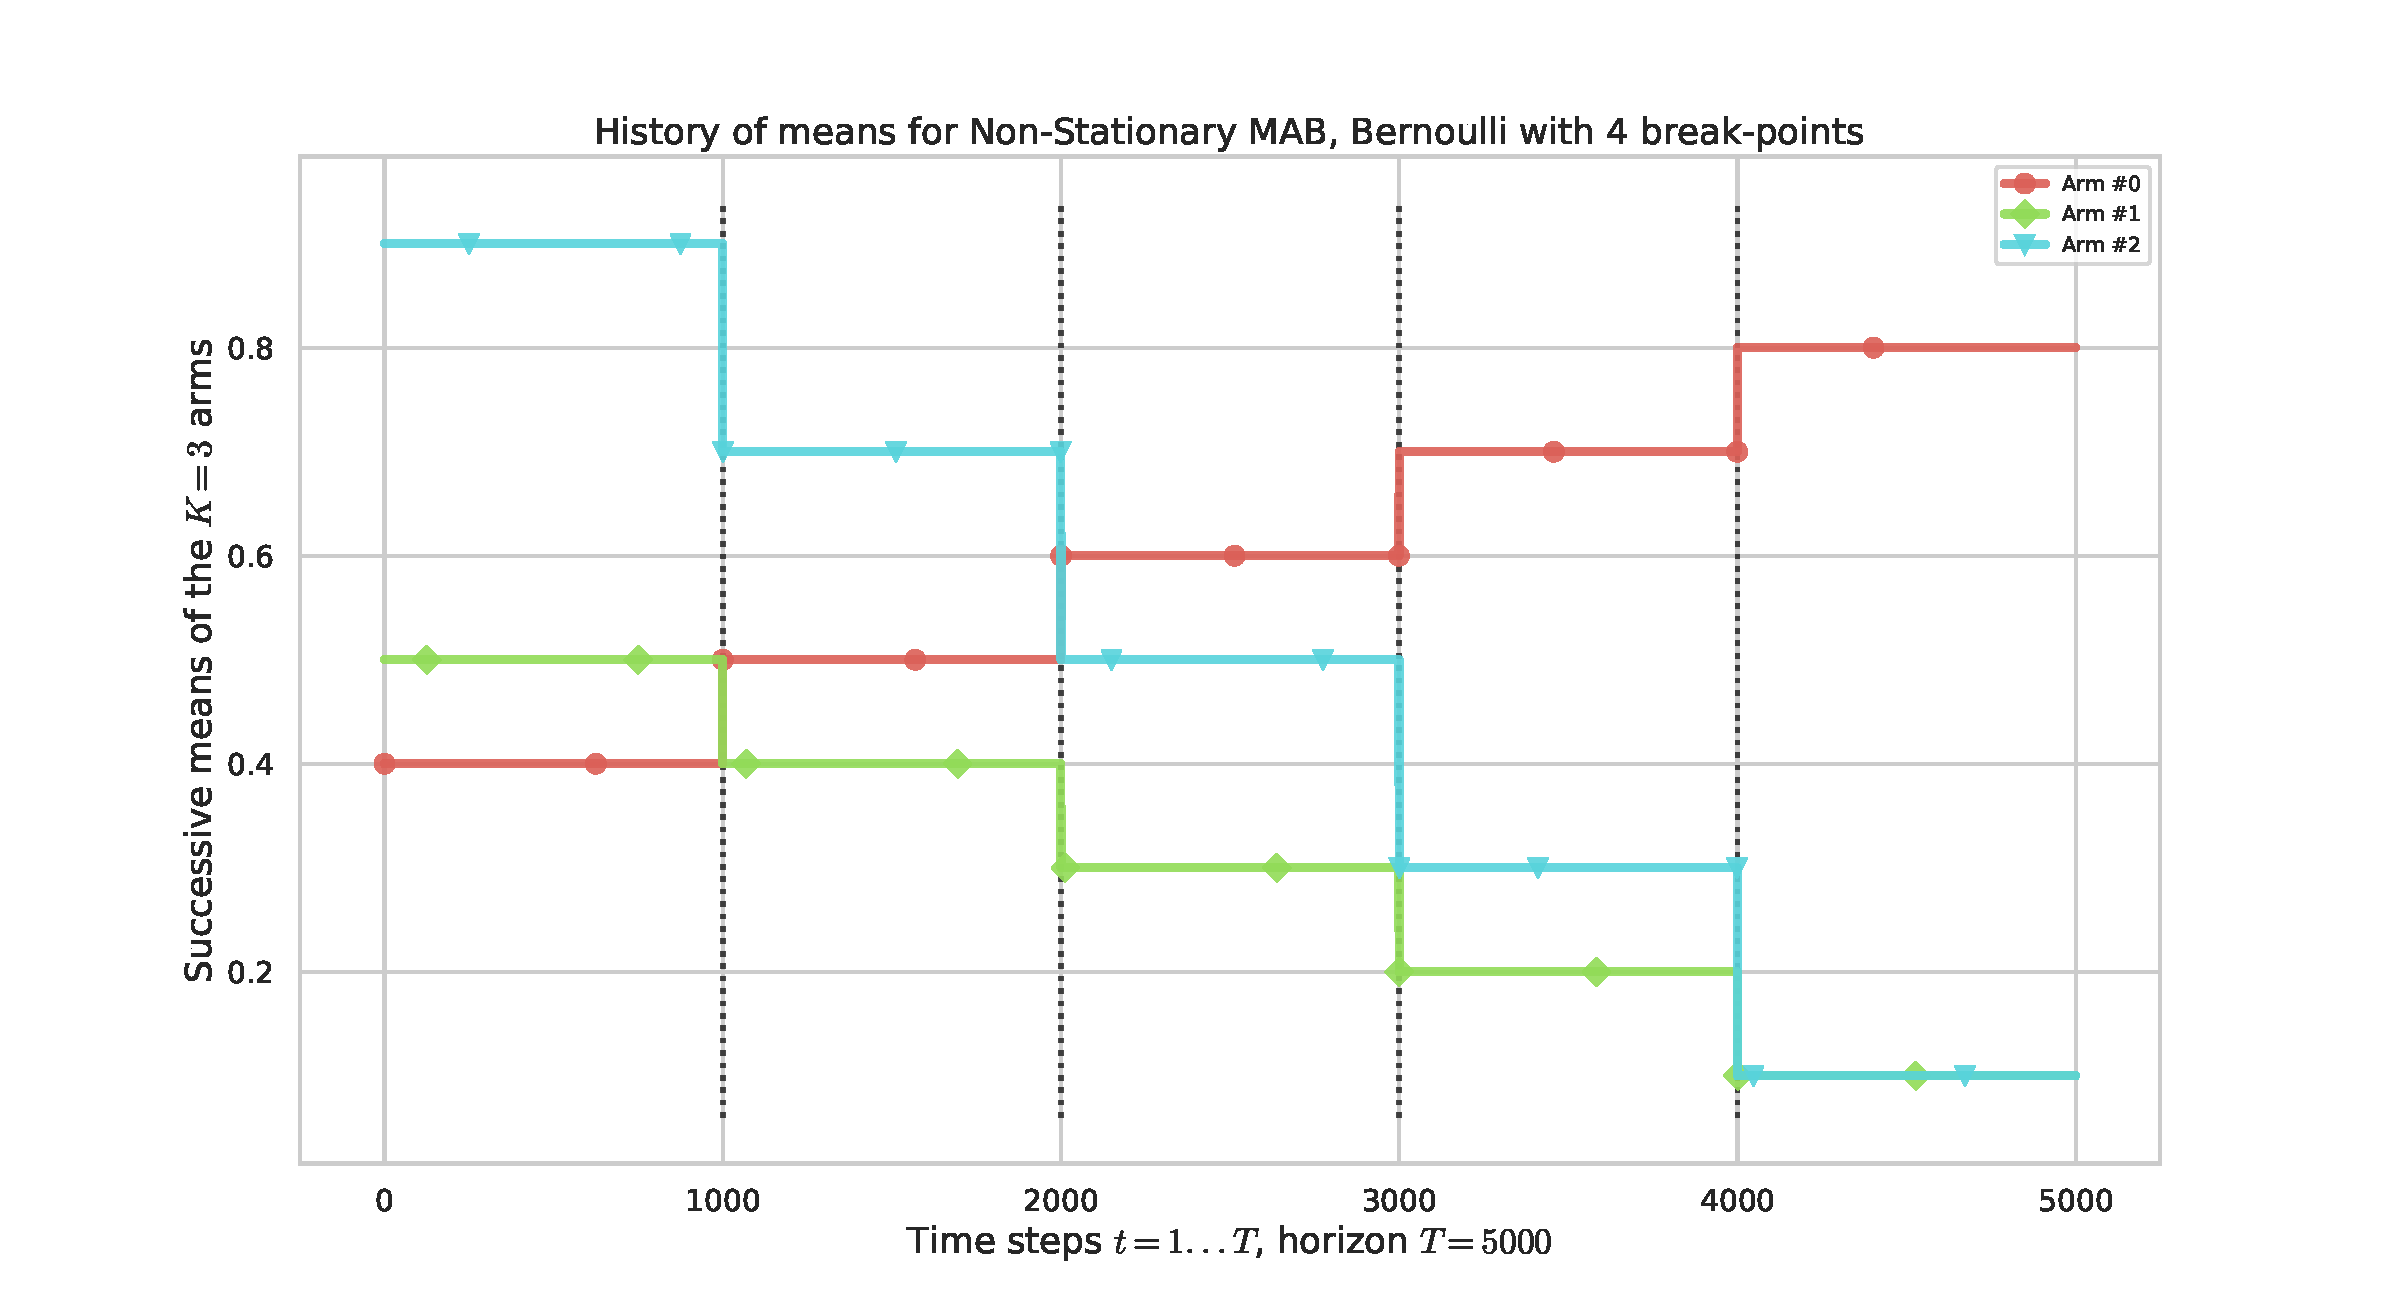
\includegraphics[width=1.00\textwidth]{figures/Problem_2.pdf}
\end{frame}

\begin{frame}[plain]{Results on problem 2}
  \centering
  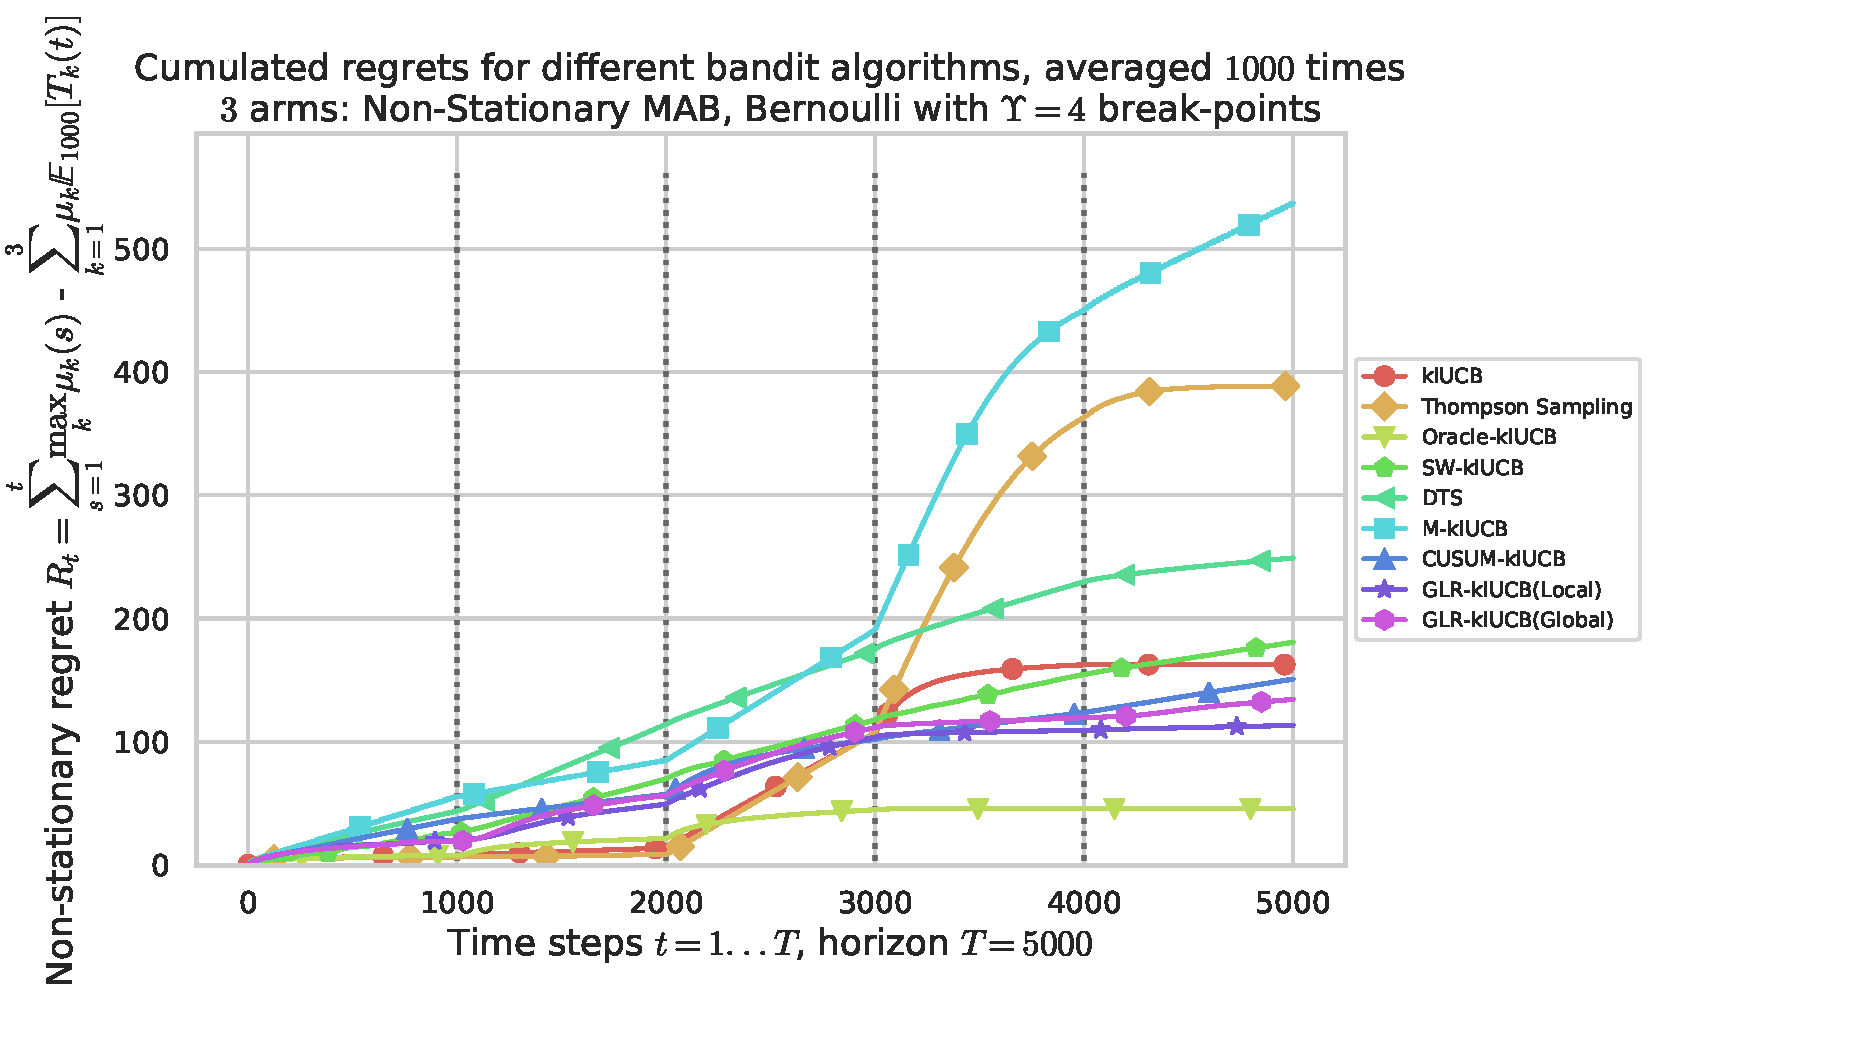
\includegraphics[width=1.05\textwidth]{figures/regret_problem2.pdf}

  $\implies$ BGLR again achieves the best performance \dCooley{} !
\end{frame}


\begin{frame}[plain]{Pb 3: non-uniform lenghts of stationary sequences}
  \centering
  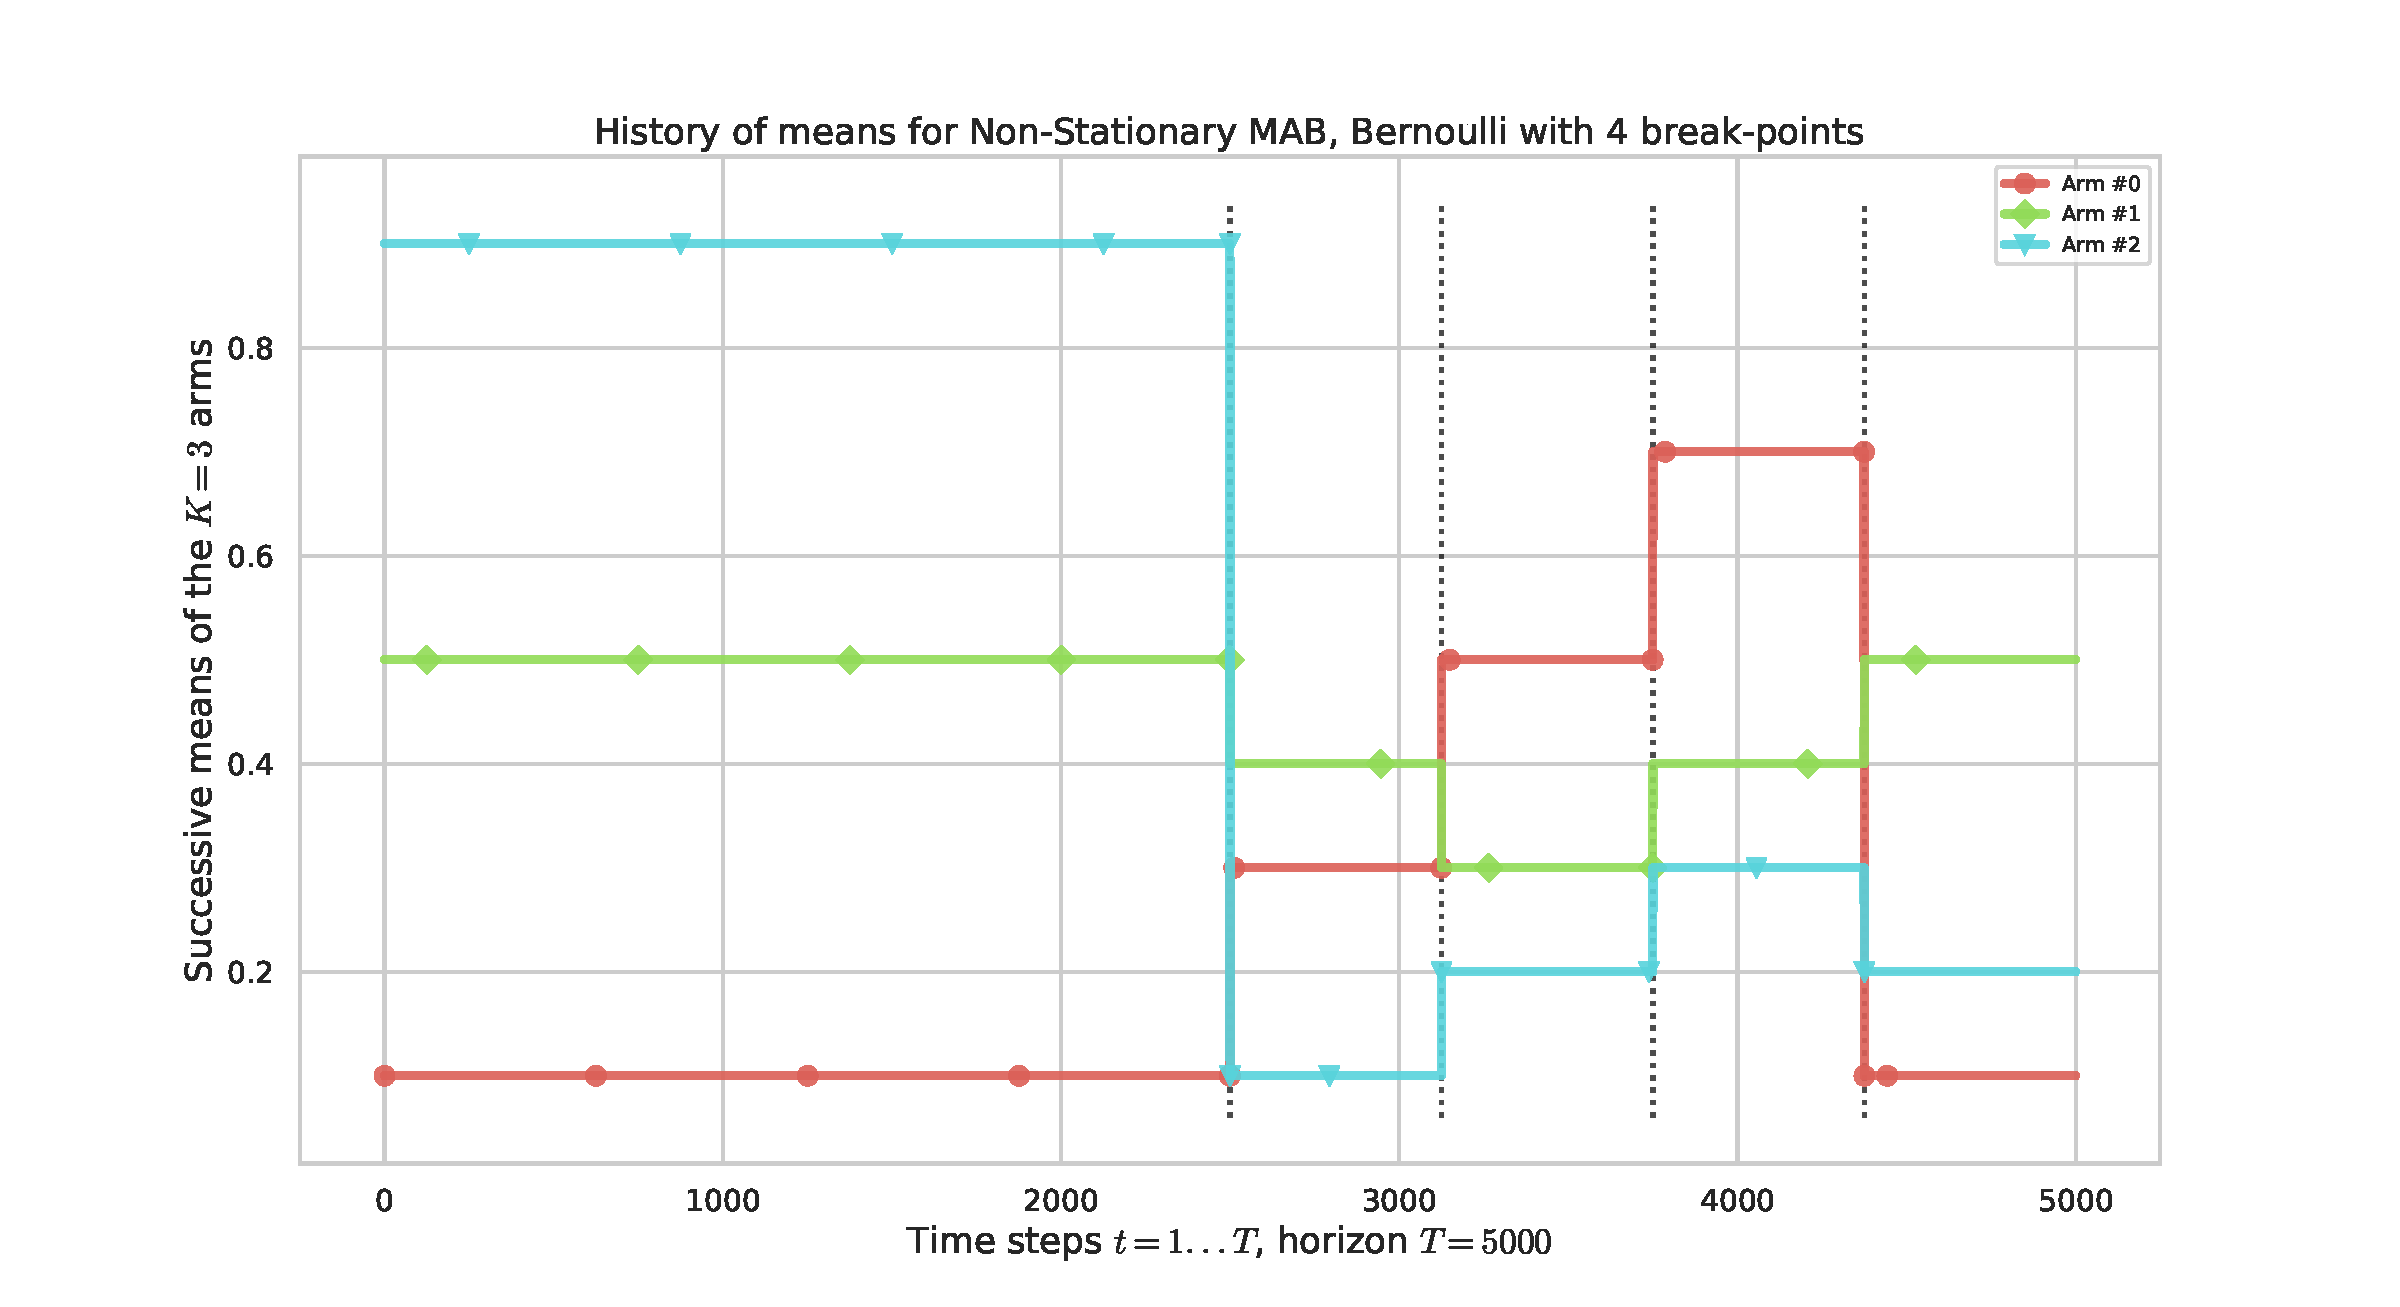
\includegraphics[width=1.00\textwidth]{figures/Problem_4.pdf}
\end{frame}

\begin{frame}[plain]{Results on problem 3}
  \centering
  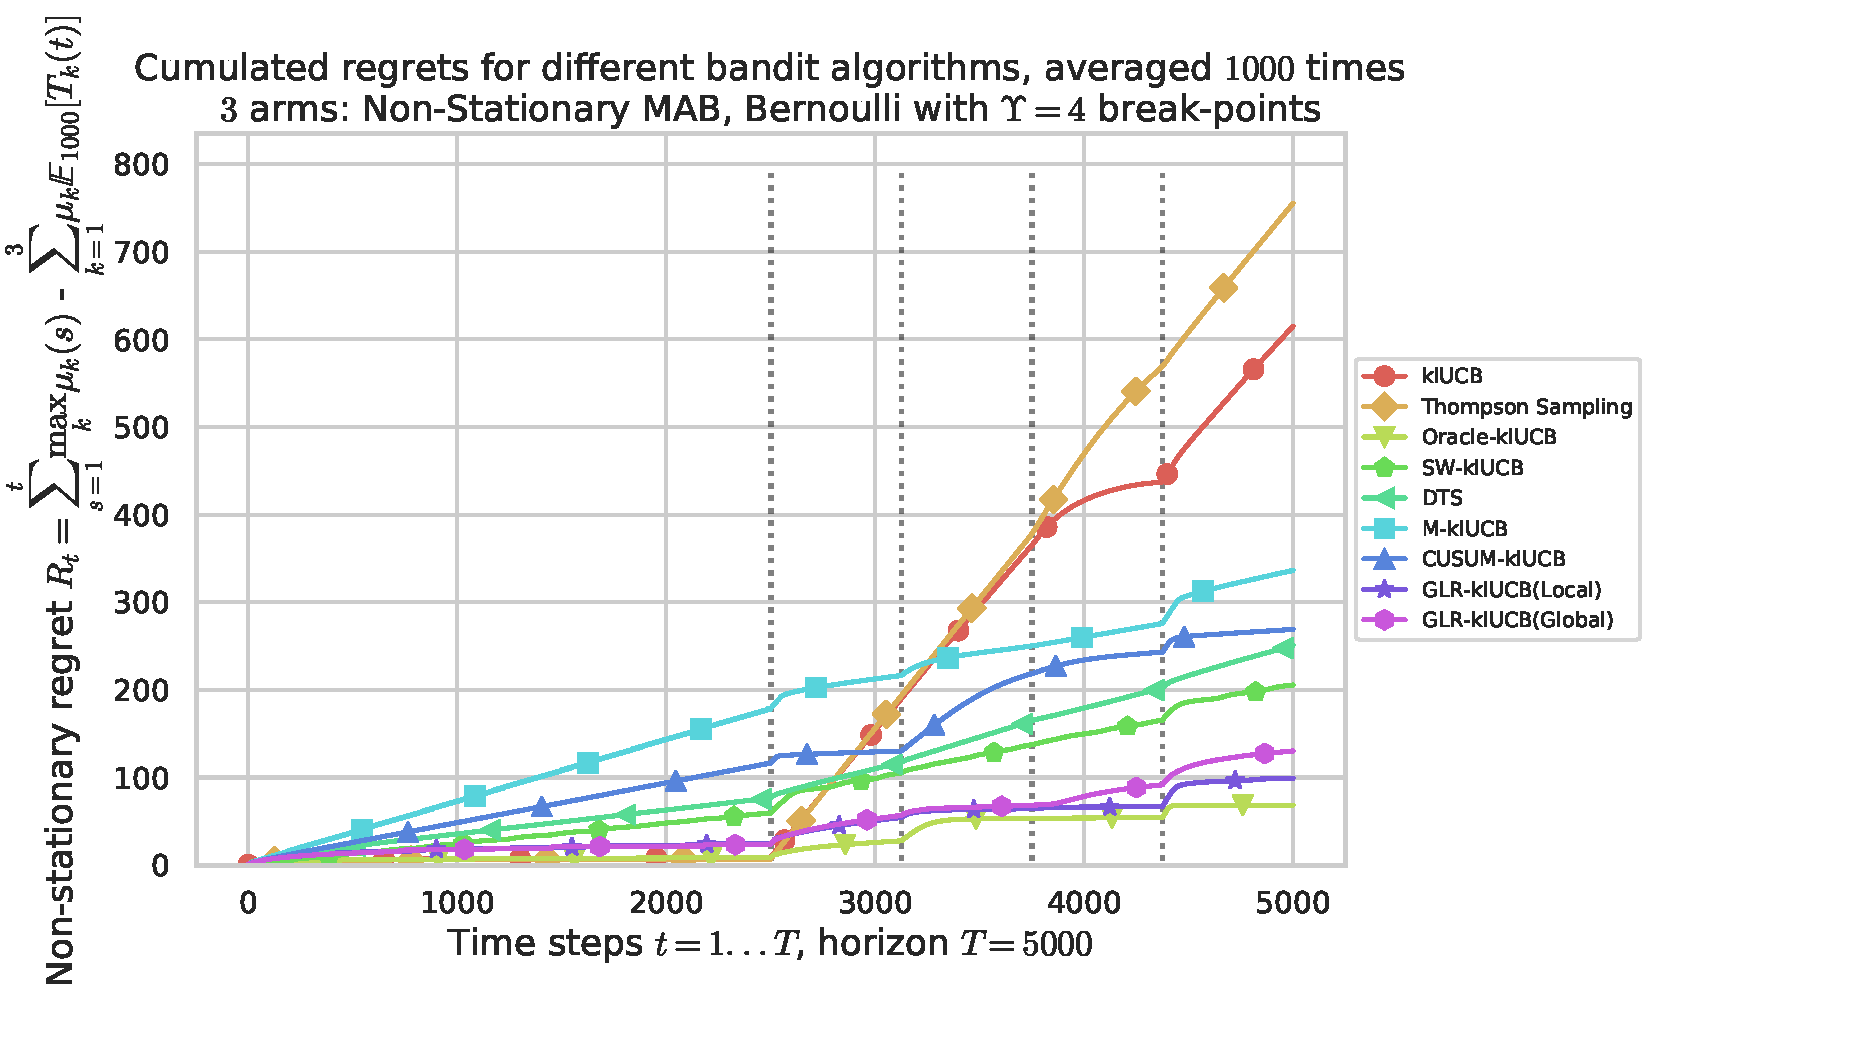
\includegraphics[width=1.05\textwidth]{figures/regret_problem4.pdf}

  $\implies$ BGLR achieves the best performance among non-oracle algorithms \dCooley{} !
\end{frame}


\subsection{\hfill{}Conclusions from the simulations\hfill{}}

\begin{frame}{Interpretation of the simulations (1/2)}

  \begin{block}{Conclusions in terms of regret}
    \begin{itemize}
      \item
      Empirically we can check that the \alert{BGLR test is efficient} \dCooley{} :
      \begin{itemize}\tightlist
        \item
        it has a \alert{low false alarm probability},
        \item
        it has a \alert{small delay} if the stationary sequences are long enough.
      \end{itemize}
      And this is true even outside of the hypotheses of our analysis
      \item
      Using the kl-UCB indexes policy gives good performance \dCooley{}
    \end{itemize}
    $\implies$ Our algorithm (BGLR test + kl-UCB) is efficient

    $\implies$ We verified that it obtains state-of-the-art performance!
  \end{block}

\end{frame}


\begin{frame}{Interpretation of the simulations (2/2)}

  What about the efficiency in terms of \textcolor{blue}{memory} and \alert{time} complexity?

  \begin{block}{Memory: efficient \dSmiley}
    Our algorithm is as efficient as other state-of-the-art strategies!\\
    \textcolor{gray}{Memory cost $= \mathcal{O}(K d_{\max})$ for $K$ arms.}
  \end{block}

  \begin{alertblock}<2->{Time: slow \dSadey{} !}
    But it is too slow!
    Time cost $= \mathcal{O}(K d_{\max} \alert{\times t})$
    at every time step $t$,
    % for $K$ arms.
    so $\mathcal{O}(K d_{\max} \alert{T^2})$ in total.
    %  and horizon $T$.

    $\hookrightarrow$ we proposed two numerical tweaks to speed it up

    $\implies$ BGLR test + kl-UCB can be as fast as M-UCB or CUSUM-UCB
    % , the two algorithms that perform as well in terms of regret

    % \hfill{} See the long version on \href{https://hal.inria.fr/hal-02006471}{\textcolor{blue}{HAL-02006471}} and \href{https://arxiv.org/abs/1902.01575}{\textcolor{blue}{arXiv:1902.01575}}
  \end{alertblock}

  \begin{small}
    ($d_{\max} = \max\limits_i \tau^i - \tau^{i+1} =$ duration of the longer stationary sequence)
    % , $T \leq (1+\Upsilon_T) d_{\max}$)
  \end{small}

\end{frame}



\section{\hfill{}Conclusion\hfill{}}
\subsection{Summary}

\begin{frame}{Summary}

  What we just presented\ldots{}
  \begin{itemize}
    \item
    Stationary or \alert{piece-wise stationary} Multi-Armed Bandits problems
    %  (MAB)
    \item
    The efficient Bernoulli Generalized Likelihood Ratio test \dCooley{}
    % (B-GLRT)
    \begin{itemize}\tightlist
      \item
      to detect break-points with \alert{no false alarm} and \alert{low delay}
      \item
      for Bernoulli data, and can also be used for sub-Bernoulli data (any bounded distributions),
      \item
      and does \emph{not} need to know the amplitude of the break-point
    \end{itemize}
    \item
    We can combine it with an efficient MAB policy:
    \alert{BGLR + kl-UCB}  \dCooley{}
    \item
    Its regret bound is $R_T = \mathcal{O}(K \sqrt{T \Upsilon_T \log(T)})$  \dCooley{} (state-of-the-art)
    \item
    Our algorithm outperforms other efficient policies on numerical simulations \dCooley\\
    and BGLR + kl-UCB can be as fast as its best competitors.
  \end{itemize}

\end{frame}

\subsection{Merci}
\begin{frame}{Conclusion}

\begin{center}
  \begin{Large}
    {\Fontify Merci de votre attention.}
    \Innocey[1.2]
  \end{Large}
\end{center}

\vspace*{20pt}

\begin{center}
  \begin{Large}
    Questions \& Discussion ?
  \end{Large}
\end{center}

\end{frame}

\end{document}
